\documentclass[twoside]{book}

% Packages required by doxygen
\usepackage{calc}
\usepackage{doxygen}
\usepackage{graphicx}
\usepackage[utf8]{inputenc}
\usepackage{makeidx}
\usepackage{multicol}
\usepackage{multirow}
\usepackage{textcomp}
\usepackage[table]{xcolor}

% Font selection
\usepackage[T1]{fontenc}
\usepackage{mathptmx}
\usepackage[scaled=.90]{helvet}
\usepackage{courier}
\usepackage{amssymb}
\usepackage{sectsty}
\renewcommand{\familydefault}{\sfdefault}
\allsectionsfont{%
  \fontseries{bc}\selectfont%
  \color{darkgray}%
}
\renewcommand{\DoxyLabelFont}{%
  \fontseries{bc}\selectfont%
  \color{darkgray}%
}

% Page & text layout
\usepackage{geometry}
\geometry{%
  a4paper,%
  top=2.5cm,%
  bottom=2.5cm,%
  left=2.5cm,%
  right=2.5cm%
}
\tolerance=750
\hfuzz=15pt
\hbadness=750
\setlength{\emergencystretch}{15pt}
\setlength{\parindent}{0cm}
\setlength{\parskip}{0.2cm}
\makeatletter
\renewcommand{\paragraph}{%
  \@startsection{paragraph}{4}{0ex}{-1.0ex}{1.0ex}{%
    \normalfont\normalsize\bfseries\SS@parafont%
  }%
}
\renewcommand{\subparagraph}{%
  \@startsection{subparagraph}{5}{0ex}{-1.0ex}{1.0ex}{%
    \normalfont\normalsize\bfseries\SS@subparafont%
  }%
}
\makeatother

% Headers & footers
\usepackage{fancyhdr}
\pagestyle{fancyplain}
\fancyhead[LE]{\fancyplain{}{\bfseries\thepage}}
\fancyhead[CE]{\fancyplain{}{}}
\fancyhead[RE]{\fancyplain{}{\bfseries\leftmark}}
\fancyhead[LO]{\fancyplain{}{\bfseries\rightmark}}
\fancyhead[CO]{\fancyplain{}{}}
\fancyhead[RO]{\fancyplain{}{\bfseries\thepage}}
\fancyfoot[LE]{\fancyplain{}{}}
\fancyfoot[CE]{\fancyplain{}{}}
\fancyfoot[RE]{\fancyplain{}{\bfseries\scriptsize Generated on Sat Apr 19 2014 15\-:44\-:02 for A\-E\-S Visualizer by Doxygen }}
\fancyfoot[LO]{\fancyplain{}{\bfseries\scriptsize Generated on Sat Apr 19 2014 15\-:44\-:02 for A\-E\-S Visualizer by Doxygen }}
\fancyfoot[CO]{\fancyplain{}{}}
\fancyfoot[RO]{\fancyplain{}{}}
\renewcommand{\footrulewidth}{0.4pt}
\renewcommand{\chaptermark}[1]{%
  \markboth{#1}{}%
}
\renewcommand{\sectionmark}[1]{%
  \markright{\thesection\ #1}%
}

% Indices & bibliography
\usepackage{natbib}
\usepackage[titles]{tocloft}
\setcounter{tocdepth}{3}
\setcounter{secnumdepth}{5}
\makeindex

% Hyperlinks (required, but should be loaded last)
\usepackage{ifpdf}
\ifpdf
  \usepackage[pdftex,pagebackref=true]{hyperref}
\else
  \usepackage[ps2pdf,pagebackref=true]{hyperref}
\fi
\hypersetup{%
  colorlinks=true,%
  linkcolor=blue,%
  citecolor=blue,%
  unicode%
}

% Custom commands
\newcommand{\clearemptydoublepage}{%
  \newpage{\pagestyle{empty}\cleardoublepage}%
}


%===== C O N T E N T S =====

\begin{document}

% Titlepage & ToC
\hypersetup{pageanchor=false}
\pagenumbering{roman}
\begin{titlepage}
\vspace*{7cm}
\begin{center}%
{\Large A\-E\-S Visualizer \\[1ex]\large 1.\-0 }\\
\vspace*{1cm}
{\large Generated by Doxygen 1.8.5}\\
\vspace*{0.5cm}
{\small Sat Apr 19 2014 15:44:02}\\
\end{center}
\end{titlepage}
\clearemptydoublepage
\tableofcontents
\clearemptydoublepage
\pagenumbering{arabic}
\hypersetup{pageanchor=true}

%--- Begin generated contents ---
\chapter{Visual\-A\-E\-S}
\label{md__r_e_a_d_m_e}
\hypertarget{md__r_e_a_d_m_e}{}
Simple how-\/to-\/setup\-: In the package we received from Blake, you want to run Py\-Scripter (It's actually pretty good from what I can tell). Now, you want to open up the simplegui.\-py. Now push run. It should work. If it doesn't, Google/\-Bing the problem. Enjoy. 
\chapter{Hierarchical Index}
\section{Class Hierarchy}
This inheritance list is sorted roughly, but not completely, alphabetically\-:\begin{DoxyCompactList}
\item \contentsline{section}{setup.\-Build\-Exe}{\pageref{classsetup_1_1_build_exe}}{}
\item object\begin{DoxyCompactList}
\item \contentsline{section}{entropy.\-Entropy}{\pageref{classentropy_1_1_entropy}}{}
\item \contentsline{section}{simplegui2.\-History\-Point}{\pageref{classsimplegui2_1_1_history_point}}{}
\item \contentsline{section}{simplegui3.\-History\-Point}{\pageref{classsimplegui3_1_1_history_point}}{}
\item \contentsline{section}{simplegui.\-History\-Point}{\pageref{classsimplegui_1_1_history_point}}{}
\item \contentsline{section}{slowaes.\-A\-E\-S}{\pageref{classslowaes_1_1_a_e_s}}{}
\item \contentsline{section}{slowaes.\-A\-E\-S\-Mode\-Of\-Operation}{\pageref{classslowaes_1_1_a_e_s_mode_of_operation}}{}
\end{DoxyCompactList}
\item py2exe\begin{DoxyCompactList}
\item \contentsline{section}{setup.\-pygame2exe}{\pageref{classsetup_1_1pygame2exe}}{}
\end{DoxyCompactList}
\item Scene\begin{DoxyCompactList}
\item \contentsline{section}{simplegui2.\-Main\-Scene}{\pageref{classsimplegui2_1_1_main_scene}}{}
\item \contentsline{section}{simplegui3.\-Main\-Scene}{\pageref{classsimplegui3_1_1_main_scene}}{}
\item \contentsline{section}{simplegui.\-Main\-Scene}{\pageref{classsimplegui_1_1_main_scene}}{}
\end{DoxyCompactList}
\end{DoxyCompactList}

\chapter{Class Index}
\section{Class List}
Here are the classes, structs, unions and interfaces with brief descriptions\-:\begin{DoxyCompactList}
\item\contentsline{section}{\hyperlink{classslowaes_1_1_a_e_s}{slowaes.\-A\-E\-S} }{\pageref{classslowaes_1_1_a_e_s}}{}
\item\contentsline{section}{\hyperlink{classslowaes_1_1_a_e_s_mode_of_operation}{slowaes.\-A\-E\-S\-Mode\-Of\-Operation} }{\pageref{classslowaes_1_1_a_e_s_mode_of_operation}}{}
\item\contentsline{section}{\hyperlink{classsetup_1_1_build_exe}{setup.\-Build\-Exe} }{\pageref{classsetup_1_1_build_exe}}{}
\item\contentsline{section}{\hyperlink{classentropy_1_1_entropy}{entropy.\-Entropy} }{\pageref{classentropy_1_1_entropy}}{}
\item\contentsline{section}{\hyperlink{classsimplegui3_1_1_history_point}{simplegui3.\-History\-Point} }{\pageref{classsimplegui3_1_1_history_point}}{}
\item\contentsline{section}{\hyperlink{classsimplegui_1_1_history_point}{simplegui.\-History\-Point} \\*This marks a point in history }{\pageref{classsimplegui_1_1_history_point}}{}
\item\contentsline{section}{\hyperlink{classsimplegui2_1_1_history_point}{simplegui2.\-History\-Point} }{\pageref{classsimplegui2_1_1_history_point}}{}
\item\contentsline{section}{\hyperlink{classsimplegui3_1_1_main_scene}{simplegui3.\-Main\-Scene} }{\pageref{classsimplegui3_1_1_main_scene}}{}
\item\contentsline{section}{\hyperlink{classsimplegui_1_1_main_scene}{simplegui.\-Main\-Scene} \\*A Scene object, from the pygameui library }{\pageref{classsimplegui_1_1_main_scene}}{}
\item\contentsline{section}{\hyperlink{classsimplegui2_1_1_main_scene}{simplegui2.\-Main\-Scene} }{\pageref{classsimplegui2_1_1_main_scene}}{}
\item\contentsline{section}{\hyperlink{classsetup_1_1pygame2exe}{setup.\-pygame2exe} }{\pageref{classsetup_1_1pygame2exe}}{}
\end{DoxyCompactList}

\chapter{Class Documentation}
\hypertarget{classslowaes_1_1_a_e_s}{\section{slowaes.\-A\-E\-S Class Reference}
\label{classslowaes_1_1_a_e_s}\index{slowaes.\-A\-E\-S@{slowaes.\-A\-E\-S}}
}
Inheritance diagram for slowaes.\-A\-E\-S\-:\begin{figure}[H]
\begin{center}
\leavevmode
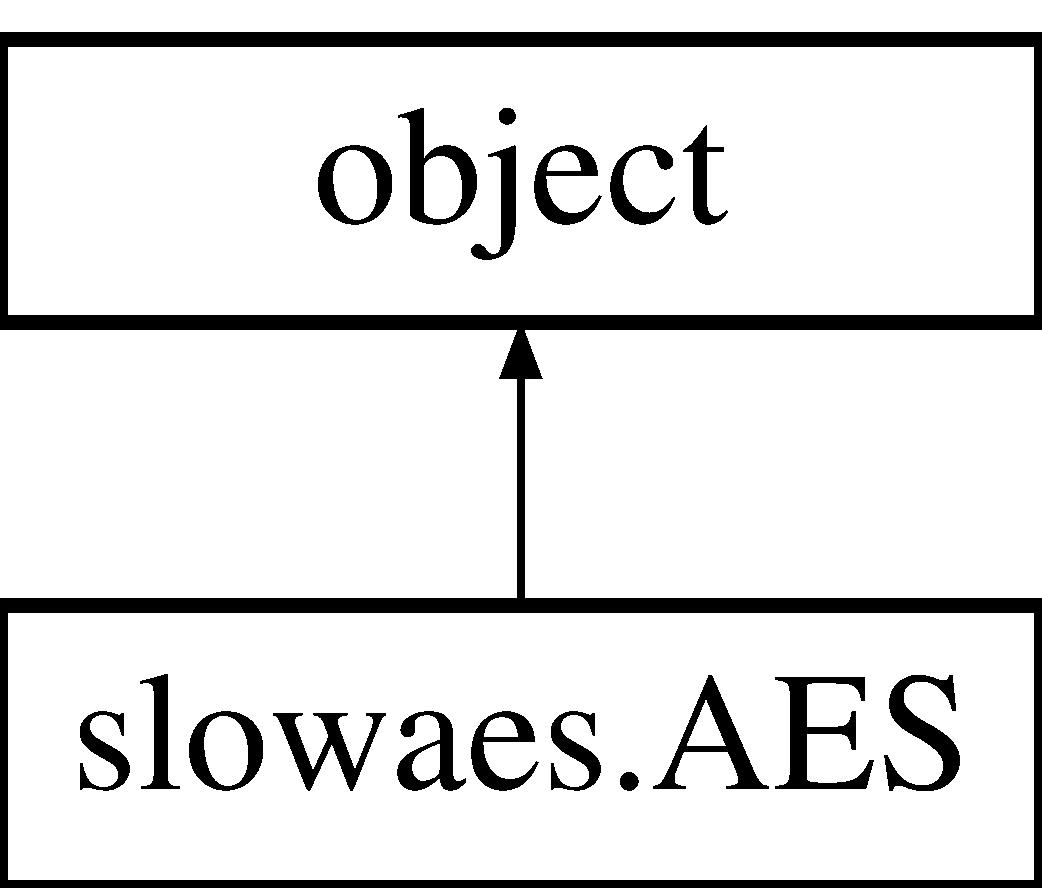
\includegraphics[height=2.000000cm]{classslowaes_1_1_a_e_s}
\end{center}
\end{figure}
\subsection*{Public Member Functions}
\begin{DoxyCompactItemize}
\item 
def \hyperlink{classslowaes_1_1_a_e_s_aa2c1b93af3bc1093e49da43396d7c185}{get\-S\-Box\-Value}
\item 
def \hyperlink{classslowaes_1_1_a_e_s_ae05b5fd6c0ba34f0ae12bda1032de765}{get\-S\-Box\-Invert}
\item 
def \hyperlink{classslowaes_1_1_a_e_s_a120952cf1cdadf630d354c9f5d486827}{rotate}
\item 
def \hyperlink{classslowaes_1_1_a_e_s_aeb77801bcddcfaf773411f1ed1de7cf0}{get\-Rcon\-Value}
\item 
def \hyperlink{classslowaes_1_1_a_e_s_a3260f08a895b18ac4d3c6ed64399c381}{core}
\item 
def \hyperlink{classslowaes_1_1_a_e_s_aab63d9aae74c2dde845f6c141c442fff}{expand\-Key}
\item 
def \hyperlink{classslowaes_1_1_a_e_s_a0ecc6c884f8e17c638ecb395bd4c7451}{add\-Round\-Key}
\item 
def \hyperlink{classslowaes_1_1_a_e_s_a97806d5c92847ff95c633154c0999557}{create\-Round\-Key}
\item 
def \hyperlink{classslowaes_1_1_a_e_s_af4dc67c05476fc947a6cd63ba7ff181f}{galois\-\_\-multiplication}
\item 
\hypertarget{classslowaes_1_1_a_e_s_a5c32f6d6aa8ae610ee82df3d426343f0}{def {\bfseries sub\-Bytes}}\label{classslowaes_1_1_a_e_s_a5c32f6d6aa8ae610ee82df3d426343f0}

\item 
\hypertarget{classslowaes_1_1_a_e_s_adeecbb0fad271f759c45765a9975dab7}{def {\bfseries shift\-Rows}}\label{classslowaes_1_1_a_e_s_adeecbb0fad271f759c45765a9975dab7}

\item 
\hypertarget{classslowaes_1_1_a_e_s_ae0586d29742a343fc50272c3219789d7}{def {\bfseries shift\-Row}}\label{classslowaes_1_1_a_e_s_ae0586d29742a343fc50272c3219789d7}

\item 
\hypertarget{classslowaes_1_1_a_e_s_a41996a1feabe5619414beffff68064d2}{def {\bfseries mix\-Columns}}\label{classslowaes_1_1_a_e_s_a41996a1feabe5619414beffff68064d2}

\item 
\hypertarget{classslowaes_1_1_a_e_s_ace6afd6a0442d9e4d812e117d9d8242c}{def {\bfseries mix\-Column}}\label{classslowaes_1_1_a_e_s_ace6afd6a0442d9e4d812e117d9d8242c}

\item 
\hypertarget{classslowaes_1_1_a_e_s_a5992fa8d15053642fd7d9d8c5a3c5540}{def {\bfseries aes\-\_\-round}}\label{classslowaes_1_1_a_e_s_a5992fa8d15053642fd7d9d8c5a3c5540}

\item 
\hypertarget{classslowaes_1_1_a_e_s_aad02794fa7ed1accc7581d76300ce8f5}{def {\bfseries aes\-\_\-inv\-Round}}\label{classslowaes_1_1_a_e_s_aad02794fa7ed1accc7581d76300ce8f5}

\item 
\hypertarget{classslowaes_1_1_a_e_s_a13dd8f92140cd60bea960d791ba5183d}{def {\bfseries aes\-\_\-main}}\label{classslowaes_1_1_a_e_s_a13dd8f92140cd60bea960d791ba5183d}

\item 
\hypertarget{classslowaes_1_1_a_e_s_aba8a4f1107bd444dd98c9028fd013c04}{def {\bfseries aes\-\_\-inv\-Main}}\label{classslowaes_1_1_a_e_s_aba8a4f1107bd444dd98c9028fd013c04}

\item 
\hypertarget{classslowaes_1_1_a_e_s_a74568e45c5071460243f2622941fe490}{def {\bfseries encrypt}}\label{classslowaes_1_1_a_e_s_a74568e45c5071460243f2622941fe490}

\item 
\hypertarget{classslowaes_1_1_a_e_s_ad85d79a9c0088dc46b4268cae8e2f054}{def {\bfseries decrypt}}\label{classslowaes_1_1_a_e_s_ad85d79a9c0088dc46b4268cae8e2f054}

\end{DoxyCompactItemize}
\subsection*{Public Attributes}
\begin{DoxyCompactItemize}
\item 
\hypertarget{classslowaes_1_1_a_e_s_a0467d80b43c5ecdf52449278e77213a2}{{\bfseries is\-Inv}}\label{classslowaes_1_1_a_e_s_a0467d80b43c5ecdf52449278e77213a2}

\item 
\hypertarget{classslowaes_1_1_a_e_s_a2df59652d33001ff70537bf5dbb6332b}{{\bfseries state}}\label{classslowaes_1_1_a_e_s_a2df59652d33001ff70537bf5dbb6332b}

\end{DoxyCompactItemize}
\subsection*{Static Public Attributes}
\begin{DoxyCompactItemize}
\item 
\hypertarget{classslowaes_1_1_a_e_s_a0c4485dde2ec4bb0a3d80e8ccad93836}{tuple {\bfseries key\-Size} = dict(S\-I\-Z\-E\-\_\-128=16, S\-I\-Z\-E\-\_\-192=24, S\-I\-Z\-E\-\_\-256=32)}\label{classslowaes_1_1_a_e_s_a0c4485dde2ec4bb0a3d80e8ccad93836}

\item 
list {\bfseries sbox}
\item 
list {\bfseries rsbox}
\item 
list {\bfseries Rcon}
\end{DoxyCompactItemize}


\subsection{Member Function Documentation}
\hypertarget{classslowaes_1_1_a_e_s_a0ecc6c884f8e17c638ecb395bd4c7451}{\index{slowaes\-::\-A\-E\-S@{slowaes\-::\-A\-E\-S}!add\-Round\-Key@{add\-Round\-Key}}
\index{add\-Round\-Key@{add\-Round\-Key}!slowaes::AES@{slowaes\-::\-A\-E\-S}}
\subsubsection[{add\-Round\-Key}]{\setlength{\rightskip}{0pt plus 5cm}def slowaes.\-A\-E\-S.\-add\-Round\-Key (
\begin{DoxyParamCaption}
\item[{}]{self, }
\item[{}]{round\-Key}
\end{DoxyParamCaption}
)}}\label{classslowaes_1_1_a_e_s_a0ecc6c884f8e17c638ecb395bd4c7451}
\begin{DoxyVerb}Adds (XORs) the round key to the state.\end{DoxyVerb}
 \hypertarget{classslowaes_1_1_a_e_s_a3260f08a895b18ac4d3c6ed64399c381}{\index{slowaes\-::\-A\-E\-S@{slowaes\-::\-A\-E\-S}!core@{core}}
\index{core@{core}!slowaes::AES@{slowaes\-::\-A\-E\-S}}
\subsubsection[{core}]{\setlength{\rightskip}{0pt plus 5cm}def slowaes.\-A\-E\-S.\-core (
\begin{DoxyParamCaption}
\item[{}]{self, }
\item[{}]{word, }
\item[{}]{iteration}
\end{DoxyParamCaption}
)}}\label{classslowaes_1_1_a_e_s_a3260f08a895b18ac4d3c6ed64399c381}
\begin{DoxyVerb}Key schedule core.\end{DoxyVerb}
 \hypertarget{classslowaes_1_1_a_e_s_a97806d5c92847ff95c633154c0999557}{\index{slowaes\-::\-A\-E\-S@{slowaes\-::\-A\-E\-S}!create\-Round\-Key@{create\-Round\-Key}}
\index{create\-Round\-Key@{create\-Round\-Key}!slowaes::AES@{slowaes\-::\-A\-E\-S}}
\subsubsection[{create\-Round\-Key}]{\setlength{\rightskip}{0pt plus 5cm}def slowaes.\-A\-E\-S.\-create\-Round\-Key (
\begin{DoxyParamCaption}
\item[{}]{self, }
\item[{}]{expanded\-Key, }
\item[{}]{round\-Key\-Pointer}
\end{DoxyParamCaption}
)}}\label{classslowaes_1_1_a_e_s_a97806d5c92847ff95c633154c0999557}
\begin{DoxyVerb}Create a round key.
Creates a round key from the given expanded key and the
position within the expanded key.
\end{DoxyVerb}
 \hypertarget{classslowaes_1_1_a_e_s_aab63d9aae74c2dde845f6c141c442fff}{\index{slowaes\-::\-A\-E\-S@{slowaes\-::\-A\-E\-S}!expand\-Key@{expand\-Key}}
\index{expand\-Key@{expand\-Key}!slowaes::AES@{slowaes\-::\-A\-E\-S}}
\subsubsection[{expand\-Key}]{\setlength{\rightskip}{0pt plus 5cm}def slowaes.\-A\-E\-S.\-expand\-Key (
\begin{DoxyParamCaption}
\item[{}]{self, }
\item[{}]{key, }
\item[{}]{size, }
\item[{}]{expanded\-Key\-Size}
\end{DoxyParamCaption}
)}}\label{classslowaes_1_1_a_e_s_aab63d9aae74c2dde845f6c141c442fff}
\begin{DoxyVerb}Rijndael's key expansion.

Expands an 128,192,256 key into an 176,208,240 bytes key

expandedKey is a char list of large enough size,
key is the non-expanded key.
\end{DoxyVerb}
 \hypertarget{classslowaes_1_1_a_e_s_af4dc67c05476fc947a6cd63ba7ff181f}{\index{slowaes\-::\-A\-E\-S@{slowaes\-::\-A\-E\-S}!galois\-\_\-multiplication@{galois\-\_\-multiplication}}
\index{galois\-\_\-multiplication@{galois\-\_\-multiplication}!slowaes::AES@{slowaes\-::\-A\-E\-S}}
\subsubsection[{galois\-\_\-multiplication}]{\setlength{\rightskip}{0pt plus 5cm}def slowaes.\-A\-E\-S.\-galois\-\_\-multiplication (
\begin{DoxyParamCaption}
\item[{}]{self, }
\item[{}]{a, }
\item[{}]{b}
\end{DoxyParamCaption}
)}}\label{classslowaes_1_1_a_e_s_af4dc67c05476fc947a6cd63ba7ff181f}
\begin{DoxyVerb}Galois multiplication of 8 bit characters a and b.\end{DoxyVerb}
 \hypertarget{classslowaes_1_1_a_e_s_aeb77801bcddcfaf773411f1ed1de7cf0}{\index{slowaes\-::\-A\-E\-S@{slowaes\-::\-A\-E\-S}!get\-Rcon\-Value@{get\-Rcon\-Value}}
\index{get\-Rcon\-Value@{get\-Rcon\-Value}!slowaes::AES@{slowaes\-::\-A\-E\-S}}
\subsubsection[{get\-Rcon\-Value}]{\setlength{\rightskip}{0pt plus 5cm}def slowaes.\-A\-E\-S.\-get\-Rcon\-Value (
\begin{DoxyParamCaption}
\item[{}]{self, }
\item[{}]{num}
\end{DoxyParamCaption}
)}}\label{classslowaes_1_1_a_e_s_aeb77801bcddcfaf773411f1ed1de7cf0}
\begin{DoxyVerb}Retrieves a given Rcon Value\end{DoxyVerb}
 \hypertarget{classslowaes_1_1_a_e_s_ae05b5fd6c0ba34f0ae12bda1032de765}{\index{slowaes\-::\-A\-E\-S@{slowaes\-::\-A\-E\-S}!get\-S\-Box\-Invert@{get\-S\-Box\-Invert}}
\index{get\-S\-Box\-Invert@{get\-S\-Box\-Invert}!slowaes::AES@{slowaes\-::\-A\-E\-S}}
\subsubsection[{get\-S\-Box\-Invert}]{\setlength{\rightskip}{0pt plus 5cm}def slowaes.\-A\-E\-S.\-get\-S\-Box\-Invert (
\begin{DoxyParamCaption}
\item[{}]{self, }
\item[{}]{num}
\end{DoxyParamCaption}
)}}\label{classslowaes_1_1_a_e_s_ae05b5fd6c0ba34f0ae12bda1032de765}
\begin{DoxyVerb}Retrieves a given Inverted S-Box Value\end{DoxyVerb}
 \hypertarget{classslowaes_1_1_a_e_s_aa2c1b93af3bc1093e49da43396d7c185}{\index{slowaes\-::\-A\-E\-S@{slowaes\-::\-A\-E\-S}!get\-S\-Box\-Value@{get\-S\-Box\-Value}}
\index{get\-S\-Box\-Value@{get\-S\-Box\-Value}!slowaes::AES@{slowaes\-::\-A\-E\-S}}
\subsubsection[{get\-S\-Box\-Value}]{\setlength{\rightskip}{0pt plus 5cm}def slowaes.\-A\-E\-S.\-get\-S\-Box\-Value (
\begin{DoxyParamCaption}
\item[{}]{self, }
\item[{}]{num}
\end{DoxyParamCaption}
)}}\label{classslowaes_1_1_a_e_s_aa2c1b93af3bc1093e49da43396d7c185}
\begin{DoxyVerb}Retrieves a given S-Box Value\end{DoxyVerb}
 \hypertarget{classslowaes_1_1_a_e_s_a120952cf1cdadf630d354c9f5d486827}{\index{slowaes\-::\-A\-E\-S@{slowaes\-::\-A\-E\-S}!rotate@{rotate}}
\index{rotate@{rotate}!slowaes::AES@{slowaes\-::\-A\-E\-S}}
\subsubsection[{rotate}]{\setlength{\rightskip}{0pt plus 5cm}def slowaes.\-A\-E\-S.\-rotate (
\begin{DoxyParamCaption}
\item[{}]{self, }
\item[{}]{word}
\end{DoxyParamCaption}
)}}\label{classslowaes_1_1_a_e_s_a120952cf1cdadf630d354c9f5d486827}
\begin{DoxyVerb}Rijndael's key schedule rotate operation.

Rotate a word eight bits to the left: eg, rotate(1d2c3a4f) == 2c3a4f1d
Word is an char list of size 4 (32 bits overall).
\end{DoxyVerb}
 

\subsection{Member Data Documentation}
\hypertarget{classslowaes_1_1_a_e_s_aa0babc9f3a99719fe10eb8b269ecd794}{\index{slowaes\-::\-A\-E\-S@{slowaes\-::\-A\-E\-S}!Rcon@{Rcon}}
\index{Rcon@{Rcon}!slowaes::AES@{slowaes\-::\-A\-E\-S}}
\subsubsection[{Rcon}]{\setlength{\rightskip}{0pt plus 5cm}list slowaes.\-A\-E\-S.\-Rcon\hspace{0.3cm}{\ttfamily [static]}}}\label{classslowaes_1_1_a_e_s_aa0babc9f3a99719fe10eb8b269ecd794}
{\bfseries Initial value\-:}
\begin{DoxyCode}
1 = [0x8d, 0x01, 0x02, 0x04, 0x08, 0x10, 0x20, 0x40, 0x80, 0x1b, 0x36,
2             0x6c, 0xd8, 0xab, 0x4d, 0x9a, 0x2f, 0x5e, 0xbc, 0x63, 0xc6, 0x97,
3             0x35, 0x6a, 0xd4, 0xb3, 0x7d, 0xfa, 0xef, 0xc5, 0x91, 0x39, 0x72,
4             0xe4, 0xd3, 0xbd, 0x61, 0xc2, 0x9f, 0x25, 0x4a, 0x94, 0x33, 0x66,
5             0xcc, 0x83, 0x1d, 0x3a, 0x74, 0xe8, 0xcb, 0x8d, 0x01, 0x02, 0x04,
6             0x08, 0x10, 0x20, 0x40, 0x80, 0x1b, 0x36, 0x6c, 0xd8, 0xab, 0x4d,
7             0x9a, 0x2f, 0x5e, 0xbc, 0x63, 0xc6, 0x97, 0x35, 0x6a, 0xd4, 0xb3,
8             0x7d, 0xfa, 0xef, 0xc5, 0x91, 0x39, 0x72, 0xe4, 0xd3, 0xbd, 0x61,
9             0xc2, 0x9f, 0x25, 0x4a, 0x94, 0x33, 0x66, 0xcc, 0x83, 0x1d, 0x3a,
10             0x74, 0xe8, 0xcb, 0x8d, 0x01, 0x02, 0x04, 0x08, 0x10, 0x20, 0x40,
11             0x80, 0x1b, 0x36, 0x6c, 0xd8, 0xab, 0x4d, 0x9a, 0x2f, 0x5e, 0xbc,
12             0x63, 0xc6, 0x97, 0x35, 0x6a, 0xd4, 0xb3, 0x7d, 0xfa, 0xef, 0xc5,
13             0x91, 0x39, 0x72, 0xe4, 0xd3, 0xbd, 0x61, 0xc2, 0x9f, 0x25, 0x4a,
14             0x94, 0x33, 0x66, 0xcc, 0x83, 0x1d, 0x3a, 0x74, 0xe8, 0xcb, 0x8d,
15             0x01, 0x02, 0x04, 0x08, 0x10, 0x20, 0x40, 0x80, 0x1b, 0x36, 0x6c,
16             0xd8, 0xab, 0x4d, 0x9a, 0x2f, 0x5e, 0xbc, 0x63, 0xc6, 0x97, 0x35,
17             0x6a, 0xd4, 0xb3, 0x7d, 0xfa, 0xef, 0xc5, 0x91, 0x39, 0x72, 0xe4,
18             0xd3, 0xbd, 0x61, 0xc2, 0x9f, 0x25, 0x4a, 0x94, 0x33, 0x66, 0xcc,
19             0x83, 0x1d, 0x3a, 0x74, 0xe8, 0xcb, 0x8d, 0x01, 0x02, 0x04, 0x08,
20             0x10, 0x20, 0x40, 0x80, 0x1b, 0x36, 0x6c, 0xd8, 0xab, 0x4d, 0x9a,
21             0x2f, 0x5e, 0xbc, 0x63, 0xc6, 0x97, 0x35, 0x6a, 0xd4, 0xb3, 0x7d,
22             0xfa, 0xef, 0xc5, 0x91, 0x39, 0x72, 0xe4, 0xd3, 0xbd, 0x61, 0xc2,
23             0x9f, 0x25, 0x4a, 0x94, 0x33, 0x66, 0xcc, 0x83, 0x1d, 0x3a, 0x74,
24             0xe8, 0xcb ]
\end{DoxyCode}
\hypertarget{classslowaes_1_1_a_e_s_ab854386b91e23a5a6c2b6a0fff48800f}{\index{slowaes\-::\-A\-E\-S@{slowaes\-::\-A\-E\-S}!rsbox@{rsbox}}
\index{rsbox@{rsbox}!slowaes::AES@{slowaes\-::\-A\-E\-S}}
\subsubsection[{rsbox}]{\setlength{\rightskip}{0pt plus 5cm}list slowaes.\-A\-E\-S.\-rsbox\hspace{0.3cm}{\ttfamily [static]}}}\label{classslowaes_1_1_a_e_s_ab854386b91e23a5a6c2b6a0fff48800f}
{\bfseries Initial value\-:}
\begin{DoxyCode}
1 = [0x52, 0x09, 0x6a, 0xd5, 0x30, 0x36, 0xa5, 0x38, 0xbf, 0x40, 0xa3,
2             0x9e, 0x81, 0xf3, 0xd7, 0xfb , 0x7c, 0xe3, 0x39, 0x82, 0x9b, 0x2f,
3             0xff, 0x87, 0x34, 0x8e, 0x43, 0x44, 0xc4, 0xde, 0xe9, 0xcb , 0x54,
4             0x7b, 0x94, 0x32, 0xa6, 0xc2, 0x23, 0x3d, 0xee, 0x4c, 0x95, 0x0b,
5             0x42, 0xfa, 0xc3, 0x4e , 0x08, 0x2e, 0xa1, 0x66, 0x28, 0xd9, 0x24,
6             0xb2, 0x76, 0x5b, 0xa2, 0x49, 0x6d, 0x8b, 0xd1, 0x25 , 0x72, 0xf8,
7             0xf6, 0x64, 0x86, 0x68, 0x98, 0x16, 0xd4, 0xa4, 0x5c, 0xcc, 0x5d,
8             0x65, 0xb6, 0x92 , 0x6c, 0x70, 0x48, 0x50, 0xfd, 0xed, 0xb9, 0xda,
9             0x5e, 0x15, 0x46, 0x57, 0xa7, 0x8d, 0x9d, 0x84 , 0x90, 0xd8, 0xab,
10             0x00, 0x8c, 0xbc, 0xd3, 0x0a, 0xf7, 0xe4, 0x58, 0x05, 0xb8, 0xb3,
11             0x45, 0x06 , 0xd0, 0x2c, 0x1e, 0x8f, 0xca, 0x3f, 0x0f, 0x02, 0xc1,
12             0xaf, 0xbd, 0x03, 0x01, 0x13, 0x8a, 0x6b , 0x3a, 0x91, 0x11, 0x41,
13             0x4f, 0x67, 0xdc, 0xea, 0x97, 0xf2, 0xcf, 0xce, 0xf0, 0xb4, 0xe6,
14             0x73 , 0x96, 0xac, 0x74, 0x22, 0xe7, 0xad, 0x35, 0x85, 0xe2, 0xf9,
15             0x37, 0xe8, 0x1c, 0x75, 0xdf, 0x6e , 0x47, 0xf1, 0x1a, 0x71, 0x1d,
16             0x29, 0xc5, 0x89, 0x6f, 0xb7, 0x62, 0x0e, 0xaa, 0x18, 0xbe, 0x1b ,
17             0xfc, 0x56, 0x3e, 0x4b, 0xc6, 0xd2, 0x79, 0x20, 0x9a, 0xdb, 0xc0,
18             0xfe, 0x78, 0xcd, 0x5a, 0xf4 , 0x1f, 0xdd, 0xa8, 0x33, 0x88, 0x07,
19             0xc7, 0x31, 0xb1, 0x12, 0x10, 0x59, 0x27, 0x80, 0xec, 0x5f , 0x60,
20             0x51, 0x7f, 0xa9, 0x19, 0xb5, 0x4a, 0x0d, 0x2d, 0xe5, 0x7a, 0x9f,
21             0x93, 0xc9, 0x9c, 0xef , 0xa0, 0xe0, 0x3b, 0x4d, 0xae, 0x2a, 0xf5,
22             0xb0, 0xc8, 0xeb, 0xbb, 0x3c, 0x83, 0x53, 0x99, 0x61 , 0x17, 0x2b,
23             0x04, 0x7e, 0xba, 0x77, 0xd6, 0x26, 0xe1, 0x69, 0x14, 0x63, 0x55,
24             0x21, 0x0c, 0x7d]
\end{DoxyCode}
\hypertarget{classslowaes_1_1_a_e_s_a584e03efd453993b40fef780984be0bb}{\index{slowaes\-::\-A\-E\-S@{slowaes\-::\-A\-E\-S}!sbox@{sbox}}
\index{sbox@{sbox}!slowaes::AES@{slowaes\-::\-A\-E\-S}}
\subsubsection[{sbox}]{\setlength{\rightskip}{0pt plus 5cm}list slowaes.\-A\-E\-S.\-sbox\hspace{0.3cm}{\ttfamily [static]}}}\label{classslowaes_1_1_a_e_s_a584e03efd453993b40fef780984be0bb}
{\bfseries Initial value\-:}
\begin{DoxyCode}
1 = [0x63, 0x7c, 0x77, 0x7b, 0xf2, 0x6b, 0x6f, 0xc5, 0x30, 0x01, 0x67,
2             0x2b, 0xfe, 0xd7, 0xab, 0x76, 0xca, 0x82, 0xc9, 0x7d, 0xfa, 0x59,
3             0x47, 0xf0, 0xad, 0xd4, 0xa2, 0xaf, 0x9c, 0xa4, 0x72, 0xc0, 0xb7,
4             0xfd, 0x93, 0x26, 0x36, 0x3f, 0xf7, 0xcc, 0x34, 0xa5, 0xe5, 0xf1,
5             0x71, 0xd8, 0x31, 0x15, 0x04, 0xc7, 0x23, 0xc3, 0x18, 0x96, 0x05,
6             0x9a, 0x07, 0x12, 0x80, 0xe2, 0xeb, 0x27, 0xb2, 0x75, 0x09, 0x83,
7             0x2c, 0x1a, 0x1b, 0x6e, 0x5a, 0xa0, 0x52, 0x3b, 0xd6, 0xb3, 0x29,
8             0xe3, 0x2f, 0x84, 0x53, 0xd1, 0x00, 0xed, 0x20, 0xfc, 0xb1, 0x5b,
9             0x6a, 0xcb, 0xbe, 0x39, 0x4a, 0x4c, 0x58, 0xcf, 0xd0, 0xef, 0xaa,
10             0xfb, 0x43, 0x4d, 0x33, 0x85, 0x45, 0xf9, 0x02, 0x7f, 0x50, 0x3c,
11             0x9f, 0xa8, 0x51, 0xa3, 0x40, 0x8f, 0x92, 0x9d, 0x38, 0xf5, 0xbc,
12             0xb6, 0xda, 0x21, 0x10, 0xff, 0xf3, 0xd2, 0xcd, 0x0c, 0x13, 0xec,
13             0x5f, 0x97, 0x44, 0x17, 0xc4, 0xa7, 0x7e, 0x3d, 0x64, 0x5d, 0x19,
14             0x73, 0x60, 0x81, 0x4f, 0xdc, 0x22, 0x2a, 0x90, 0x88, 0x46, 0xee,
15             0xb8, 0x14, 0xde, 0x5e, 0x0b, 0xdb, 0xe0, 0x32, 0x3a, 0x0a, 0x49,
16             0x06, 0x24, 0x5c, 0xc2, 0xd3, 0xac, 0x62, 0x91, 0x95, 0xe4, 0x79,
17             0xe7, 0xc8, 0x37, 0x6d, 0x8d, 0xd5, 0x4e, 0xa9, 0x6c, 0x56, 0xf4,
18             0xea, 0x65, 0x7a, 0xae, 0x08, 0xba, 0x78, 0x25, 0x2e, 0x1c, 0xa6,
19             0xb4, 0xc6, 0xe8, 0xdd, 0x74, 0x1f, 0x4b, 0xbd, 0x8b, 0x8a, 0x70,
20             0x3e, 0xb5, 0x66, 0x48, 0x03, 0xf6, 0x0e, 0x61, 0x35, 0x57, 0xb9,
21             0x86, 0xc1, 0x1d, 0x9e, 0xe1, 0xf8, 0x98, 0x11, 0x69, 0xd9, 0x8e,
22             0x94, 0x9b, 0x1e, 0x87, 0xe9, 0xce, 0x55, 0x28, 0xdf, 0x8c, 0xa1,
23             0x89, 0x0d, 0xbf, 0xe6, 0x42, 0x68, 0x41, 0x99, 0x2d, 0x0f, 0xb0,
24             0x54, 0xbb, 0x16]
\end{DoxyCode}


The documentation for this class was generated from the following file\-:\begin{DoxyCompactItemize}
\item 
slowaes.\-py\end{DoxyCompactItemize}

\hypertarget{classslowaes_1_1_a_e_s_mode_of_operation}{\section{slowaes.\-A\-E\-S\-Mode\-Of\-Operation Class Reference}
\label{classslowaes_1_1_a_e_s_mode_of_operation}\index{slowaes.\-A\-E\-S\-Mode\-Of\-Operation@{slowaes.\-A\-E\-S\-Mode\-Of\-Operation}}
}
Inheritance diagram for slowaes.\-A\-E\-S\-Mode\-Of\-Operation\-:\begin{figure}[H]
\begin{center}
\leavevmode
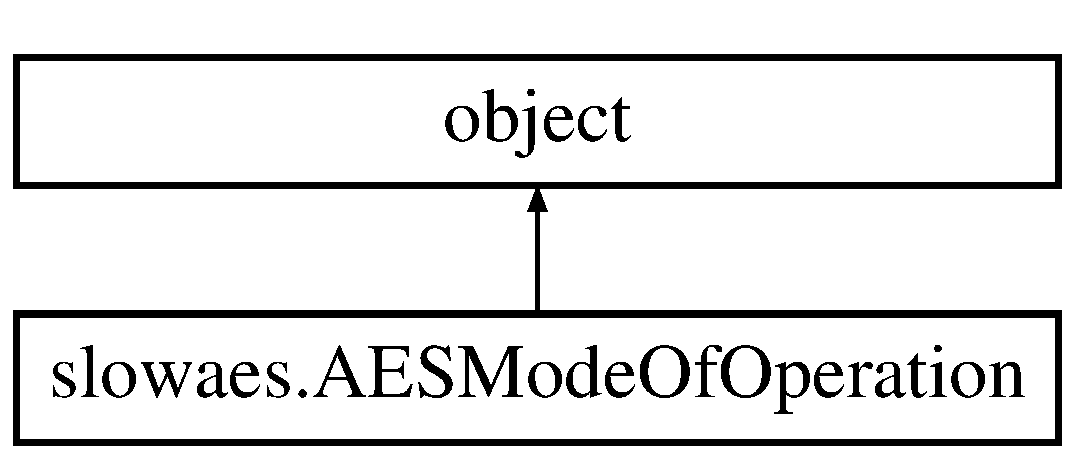
\includegraphics[height=2.000000cm]{classslowaes_1_1_a_e_s_mode_of_operation}
\end{center}
\end{figure}
\subsection*{Public Member Functions}
\begin{DoxyCompactItemize}
\item 
\hypertarget{classslowaes_1_1_a_e_s_mode_of_operation_ae5b48258fcedce545b420260d58c20df}{def {\bfseries convert\-String}}\label{classslowaes_1_1_a_e_s_mode_of_operation_ae5b48258fcedce545b420260d58c20df}

\item 
\hypertarget{classslowaes_1_1_a_e_s_mode_of_operation_a379e6dfc94dbafa6fd9d3bd9c5caa0b0}{def {\bfseries encrypt}}\label{classslowaes_1_1_a_e_s_mode_of_operation_a379e6dfc94dbafa6fd9d3bd9c5caa0b0}

\item 
\hypertarget{classslowaes_1_1_a_e_s_mode_of_operation_aa7353b4ffd4df9b274283d8a110535ed}{def {\bfseries decrypt}}\label{classslowaes_1_1_a_e_s_mode_of_operation_aa7353b4ffd4df9b274283d8a110535ed}

\end{DoxyCompactItemize}
\subsection*{Static Public Attributes}
\begin{DoxyCompactItemize}
\item 
\hypertarget{classslowaes_1_1_a_e_s_mode_of_operation_a2ba893a7e4f92bb30d43fa6c7663cc5a}{tuple {\bfseries aes} = \hyperlink{classslowaes_1_1_a_e_s}{A\-E\-S}()}\label{classslowaes_1_1_a_e_s_mode_of_operation_a2ba893a7e4f92bb30d43fa6c7663cc5a}

\item 
\hypertarget{classslowaes_1_1_a_e_s_mode_of_operation_a6c5604b7c5520fe1f35e9114132ee0c0}{tuple {\bfseries mode\-Of\-Operation} = dict(O\-F\-B=0, C\-F\-B=1, C\-B\-C=2)}\label{classslowaes_1_1_a_e_s_mode_of_operation_a6c5604b7c5520fe1f35e9114132ee0c0}

\end{DoxyCompactItemize}


The documentation for this class was generated from the following file\-:\begin{DoxyCompactItemize}
\item 
slowaes.\-py\end{DoxyCompactItemize}

\hypertarget{classsetup_1_1_build_exe}{\section{setup.\-Build\-Exe Class Reference}
\label{classsetup_1_1_build_exe}\index{setup.\-Build\-Exe@{setup.\-Build\-Exe}}
}
\subsection*{Public Member Functions}
\begin{DoxyCompactItemize}
\item 
\hypertarget{classsetup_1_1_build_exe_a84b17d860c8eb8d2d29da2f21313138b}{def {\bfseries \-\_\-\-\_\-init\-\_\-\-\_\-}}\label{classsetup_1_1_build_exe_a84b17d860c8eb8d2d29da2f21313138b}

\item 
\hypertarget{classsetup_1_1_build_exe_a30782cd3425186df73b8a116dd230104}{def \hyperlink{classsetup_1_1_build_exe_a30782cd3425186df73b8a116dd230104}{opj}}\label{classsetup_1_1_build_exe_a30782cd3425186df73b8a116dd230104}

\begin{DoxyCompactList}\small\item\em Code from Dist\-Utils tutorial at \href{http://wiki.python.org/moin/Distutils/Tutorial}{\tt http\-://wiki.\-python.\-org/moin/\-Distutils/\-Tutorial} Originally borrowed from wx\-Python's setup and config files. \end{DoxyCompactList}\item 
\hypertarget{classsetup_1_1_build_exe_ab0c85bff0ed56583e94f29867b55b26e}{def {\bfseries find\-\_\-data\-\_\-files}}\label{classsetup_1_1_build_exe_ab0c85bff0ed56583e94f29867b55b26e}

\item 
\hypertarget{classsetup_1_1_build_exe_a3541fe4525e041c9cb929754e97f4e9e}{def {\bfseries run}}\label{classsetup_1_1_build_exe_a3541fe4525e041c9cb929754e97f4e9e}

\end{DoxyCompactItemize}
\subsection*{Public Attributes}
\begin{DoxyCompactItemize}
\item 
\hypertarget{classsetup_1_1_build_exe_ab524aa075ed0f127d72c623e664e8831}{{\bfseries script}}\label{classsetup_1_1_build_exe_ab524aa075ed0f127d72c623e664e8831}

\item 
\hypertarget{classsetup_1_1_build_exe_a52313d342c9bb6b1db5faaf46bc6c6df}{{\bfseries project\-\_\-name}}\label{classsetup_1_1_build_exe_a52313d342c9bb6b1db5faaf46bc6c6df}

\item 
\hypertarget{classsetup_1_1_build_exe_a54cb1b1fbce3a1462c67e7a7a1fc27ef}{{\bfseries project\-\_\-url}}\label{classsetup_1_1_build_exe_a54cb1b1fbce3a1462c67e7a7a1fc27ef}

\item 
\hypertarget{classsetup_1_1_build_exe_ab8e79883e085c523fbd40448ffb595e9}{{\bfseries project\-\_\-version}}\label{classsetup_1_1_build_exe_ab8e79883e085c523fbd40448ffb595e9}

\item 
\hypertarget{classsetup_1_1_build_exe_ad32bc87bf6037badb4988d81c1da0acd}{{\bfseries license}}\label{classsetup_1_1_build_exe_ad32bc87bf6037badb4988d81c1da0acd}

\item 
\hypertarget{classsetup_1_1_build_exe_acbc73319da42ccadffc939368e868bf9}{{\bfseries author\-\_\-name}}\label{classsetup_1_1_build_exe_acbc73319da42ccadffc939368e868bf9}

\item 
\hypertarget{classsetup_1_1_build_exe_af8ea80871e7e6855823a686edce4540f}{{\bfseries author\-\_\-email}}\label{classsetup_1_1_build_exe_af8ea80871e7e6855823a686edce4540f}

\item 
\hypertarget{classsetup_1_1_build_exe_a7ec2b38ce15704196dc378bdb34363ee}{{\bfseries copyright}}\label{classsetup_1_1_build_exe_a7ec2b38ce15704196dc378bdb34363ee}

\item 
\hypertarget{classsetup_1_1_build_exe_ae598e335612a4263ad16730521cc4d4e}{{\bfseries project\-\_\-description}}\label{classsetup_1_1_build_exe_ae598e335612a4263ad16730521cc4d4e}

\item 
\hypertarget{classsetup_1_1_build_exe_a6c9b605d92c89a43cd64c9902a27666d}{{\bfseries icon\-\_\-file}}\label{classsetup_1_1_build_exe_a6c9b605d92c89a43cd64c9902a27666d}

\item 
\hypertarget{classsetup_1_1_build_exe_ae0edef04207e3b96a2de777b43e9ad26}{{\bfseries extra\-\_\-datas}}\label{classsetup_1_1_build_exe_ae0edef04207e3b96a2de777b43e9ad26}

\item 
\hypertarget{classsetup_1_1_build_exe_a7965e03505c7e76bfa1b66c83c6d7bcf}{{\bfseries extra\-\_\-modules}}\label{classsetup_1_1_build_exe_a7965e03505c7e76bfa1b66c83c6d7bcf}

\item 
\hypertarget{classsetup_1_1_build_exe_a62bd358704b560750febb9d4f6bf3d87}{{\bfseries exclude\-\_\-modules}}\label{classsetup_1_1_build_exe_a62bd358704b560750febb9d4f6bf3d87}

\item 
\hypertarget{classsetup_1_1_build_exe_a3661be6ceb0296d59220bc68282a5cdb}{{\bfseries exclude\-\_\-dll}}\label{classsetup_1_1_build_exe_a3661be6ceb0296d59220bc68282a5cdb}

\item 
\hypertarget{classsetup_1_1_build_exe_a911ce6dcda40696ee88b46f4d1191af6}{{\bfseries extra\-\_\-scripts}}\label{classsetup_1_1_build_exe_a911ce6dcda40696ee88b46f4d1191af6}

\item 
\hypertarget{classsetup_1_1_build_exe_a73205ec60073e573881979e1f030bc19}{{\bfseries zipfile\-\_\-name}}\label{classsetup_1_1_build_exe_a73205ec60073e573881979e1f030bc19}

\item 
\hypertarget{classsetup_1_1_build_exe_aa5d2ae97bca6ba75b0c70abeabede2d3}{{\bfseries dist\-\_\-dir}}\label{classsetup_1_1_build_exe_aa5d2ae97bca6ba75b0c70abeabede2d3}

\end{DoxyCompactItemize}


The documentation for this class was generated from the following file\-:\begin{DoxyCompactItemize}
\item 
setup.\-py\end{DoxyCompactItemize}

\hypertarget{classentropy_1_1_entropy}{\section{entropy.\-Entropy Class Reference}
\label{classentropy_1_1_entropy}\index{entropy.\-Entropy@{entropy.\-Entropy}}
}
Inheritance diagram for entropy.\-Entropy\-:\begin{figure}[H]
\begin{center}
\leavevmode
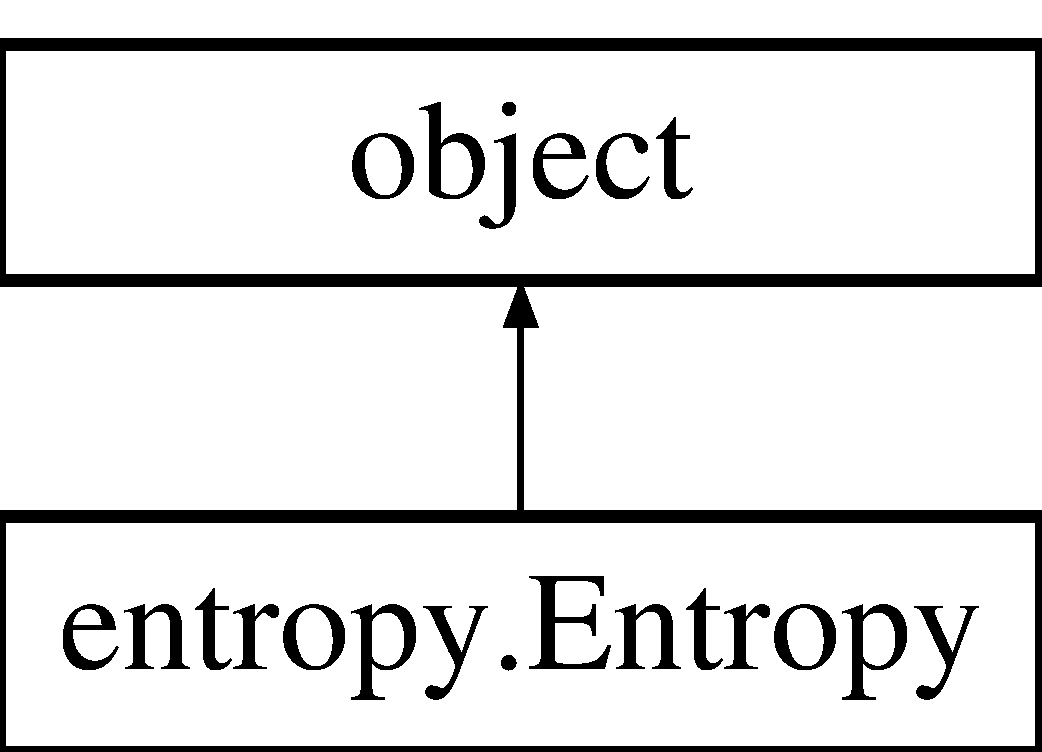
\includegraphics[height=2.000000cm]{classentropy_1_1_entropy}
\end{center}
\end{figure}
\subsection*{Public Member Functions}
\begin{DoxyCompactItemize}
\item 
\hypertarget{classentropy_1_1_entropy_a907635c50b59c160e09192fdb0cd56c5}{def {\bfseries dice\-\_\-coefficient}}\label{classentropy_1_1_entropy_a907635c50b59c160e09192fdb0cd56c5}

\item 
\hypertarget{classentropy_1_1_entropy_acc04c8428c9cd63f5f572783fefcd35f}{def {\bfseries compute\-\_\-jaccard\-\_\-index}}\label{classentropy_1_1_entropy_acc04c8428c9cd63f5f572783fefcd35f}

\item 
def \hyperlink{classentropy_1_1_entropy_a8b8657211f139161dc3851692bf496fd}{winkler\-Compare\-P}
\item 
def \hyperlink{classentropy_1_1_entropy_ab6bfc57e1b5d3b4f3fb93f243c3946cc}{get\-All\-Entropies}
\item 
def \hyperlink{classentropy_1_1_entropy_a607991156d5723944e95de617599f156}{dameraulevenshtein}
\item 
\hypertarget{classentropy_1_1_entropy_a905010113e49e5fcda39754c2d48fab4}{def {\bfseries levenshtein}}\label{classentropy_1_1_entropy_a905010113e49e5fcda39754c2d48fab4}

\end{DoxyCompactItemize}


\subsection{Detailed Description}
\begin{DoxyVerb}duplicate bigrams in a word should be counted distinctly
(per discussion), otherwise 'AA' and 'AAAA' would have a
dice coefficient of 1...
\end{DoxyVerb}
 

\subsection{Member Function Documentation}
\hypertarget{classentropy_1_1_entropy_a607991156d5723944e95de617599f156}{\index{entropy\-::\-Entropy@{entropy\-::\-Entropy}!dameraulevenshtein@{dameraulevenshtein}}
\index{dameraulevenshtein@{dameraulevenshtein}!entropy::Entropy@{entropy\-::\-Entropy}}
\subsubsection[{dameraulevenshtein}]{\setlength{\rightskip}{0pt plus 5cm}def entropy.\-Entropy.\-dameraulevenshtein (
\begin{DoxyParamCaption}
\item[{}]{self, }
\item[{}]{seq1, }
\item[{}]{seq2}
\end{DoxyParamCaption}
)}}\label{classentropy_1_1_entropy_a607991156d5723944e95de617599f156}
\begin{DoxyVerb}Calculate the Damerau-Levenshtein distance between sequences.

This distance is the number of additions, deletions, substitutions,
and transpositions needed to transform the first sequence into the
second. Although generally used with strings, any sequences of
comparable objects will work.

Transpositions are exchanges of *consecutive* characters; all other
operations are self-explanatory.

This implementation is O(N*M) time and O(M) space, for N and M the
lengths of the two sequences.

>>> dameraulevenshtein('ba', 'abc')
2
>>> dameraulevenshtein('fee', 'deed')
2

It works with arbitrary sequences too:
>>> dameraulevenshtein('abcd', ['b', 'a', 'c', 'd', 'e'])
2
\end{DoxyVerb}
 \hypertarget{classentropy_1_1_entropy_ab6bfc57e1b5d3b4f3fb93f243c3946cc}{\index{entropy\-::\-Entropy@{entropy\-::\-Entropy}!get\-All\-Entropies@{get\-All\-Entropies}}
\index{get\-All\-Entropies@{get\-All\-Entropies}!entropy::Entropy@{entropy\-::\-Entropy}}
\subsubsection[{get\-All\-Entropies}]{\setlength{\rightskip}{0pt plus 5cm}def entropy.\-Entropy.\-get\-All\-Entropies (
\begin{DoxyParamCaption}
\item[{}]{self, }
\item[{}]{one, }
\item[{}]{two}
\end{DoxyParamCaption}
)}}\label{classentropy_1_1_entropy_ab6bfc57e1b5d3b4f3fb93f243c3946cc}
\begin{DoxyVerb}one and two are the two states to compare in number array form. \end{DoxyVerb}
 \hypertarget{classentropy_1_1_entropy_a8b8657211f139161dc3851692bf496fd}{\index{entropy\-::\-Entropy@{entropy\-::\-Entropy}!winkler\-Compare\-P@{winkler\-Compare\-P}}
\index{winkler\-Compare\-P@{winkler\-Compare\-P}!entropy::Entropy@{entropy\-::\-Entropy}}
\subsubsection[{winkler\-Compare\-P}]{\setlength{\rightskip}{0pt plus 5cm}def entropy.\-Entropy.\-winkler\-Compare\-P (
\begin{DoxyParamCaption}
\item[{}]{self, }
\item[{}]{str1, }
\item[{}]{str2}
\end{DoxyParamCaption}
)}}\label{classentropy_1_1_entropy_a8b8657211f139161dc3851692bf496fd}
\begin{DoxyVerb}Return approximate string comparator measure (between 0.0 and 1.0)

USAGE:
  score = winkler(str1, str2)

ARGUMENTS:
  str1  The first string
  str2  The second string

DESCRIPTION:
  As described in 'An Application of the Fellegi-Sunter Model of
  Record Linkage to the 1990 U.S. Decennial Census' by William E. Winkler
  and Yves Thibaudeau.

  Based on the 'jaro' string comparator, but modifies it according to whether
  the first few characters are the same or not.
\end{DoxyVerb}
 

The documentation for this class was generated from the following file\-:\begin{DoxyCompactItemize}
\item 
entropy.\-py\end{DoxyCompactItemize}

\hypertarget{classsimplegui3_1_1_history_point}{\section{simplegui3.\-History\-Point Class Reference}
\label{classsimplegui3_1_1_history_point}\index{simplegui3.\-History\-Point@{simplegui3.\-History\-Point}}
}
Inheritance diagram for simplegui3.\-History\-Point\-:\begin{figure}[H]
\begin{center}
\leavevmode
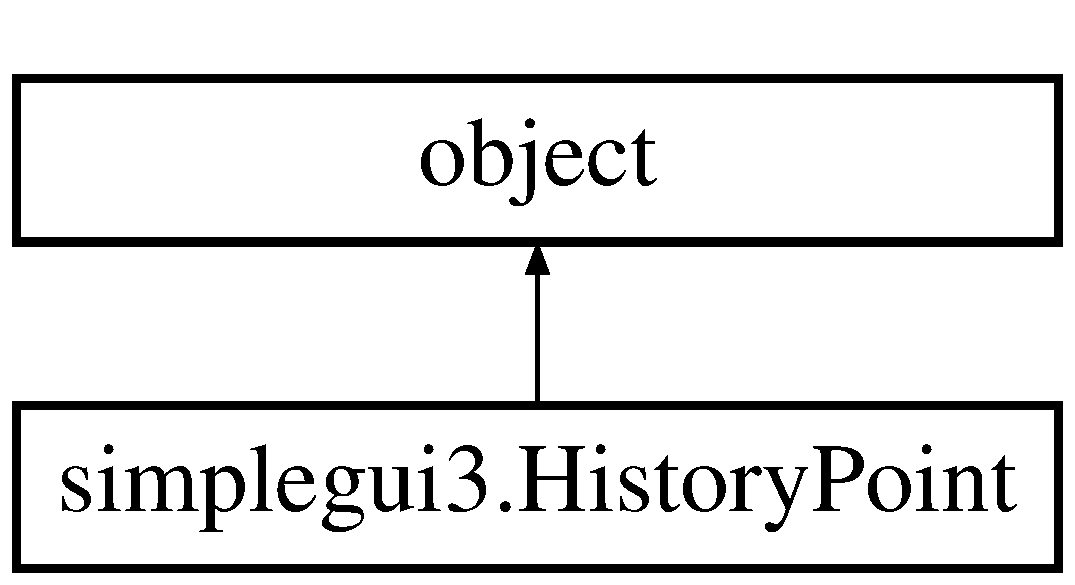
\includegraphics[height=2.000000cm]{classsimplegui3_1_1_history_point}
\end{center}
\end{figure}
\subsection*{Public Member Functions}
\begin{DoxyCompactItemize}
\item 
\hypertarget{classsimplegui3_1_1_history_point_a67048ad05a793a2f9e6c40dabc2c3f6a}{def {\bfseries \-\_\-\-\_\-init\-\_\-\-\_\-}}\label{classsimplegui3_1_1_history_point_a67048ad05a793a2f9e6c40dabc2c3f6a}

\item 
\hypertarget{classsimplegui3_1_1_history_point_a6fa9f9c36c28f45f994720c3eeb6b904}{def {\bfseries \-\_\-\-\_\-str\-\_\-\-\_\-}}\label{classsimplegui3_1_1_history_point_a6fa9f9c36c28f45f994720c3eeb6b904}

\end{DoxyCompactItemize}
\subsection*{Public Attributes}
\begin{DoxyCompactItemize}
\item 
\hypertarget{classsimplegui3_1_1_history_point_ad2f58b8ef1c0a1b0fea4e9c3ae6839f2}{{\bfseries mt}}\label{classsimplegui3_1_1_history_point_ad2f58b8ef1c0a1b0fea4e9c3ae6839f2}

\item 
\hypertarget{classsimplegui3_1_1_history_point_a2e70b601b95a033abefefcc44a746b5f}{{\bfseries mb}}\label{classsimplegui3_1_1_history_point_a2e70b601b95a033abefefcc44a746b5f}

\end{DoxyCompactItemize}


The documentation for this class was generated from the following file\-:\begin{DoxyCompactItemize}
\item 
simplegui3.\-py\end{DoxyCompactItemize}

\hypertarget{classsimplegui_1_1_history_point}{\section{simplegui.\-History\-Point Class Reference}
\label{classsimplegui_1_1_history_point}\index{simplegui.\-History\-Point@{simplegui.\-History\-Point}}
}


This marks a point in history.  


Inheritance diagram for simplegui.\-History\-Point\-:\begin{figure}[H]
\begin{center}
\leavevmode
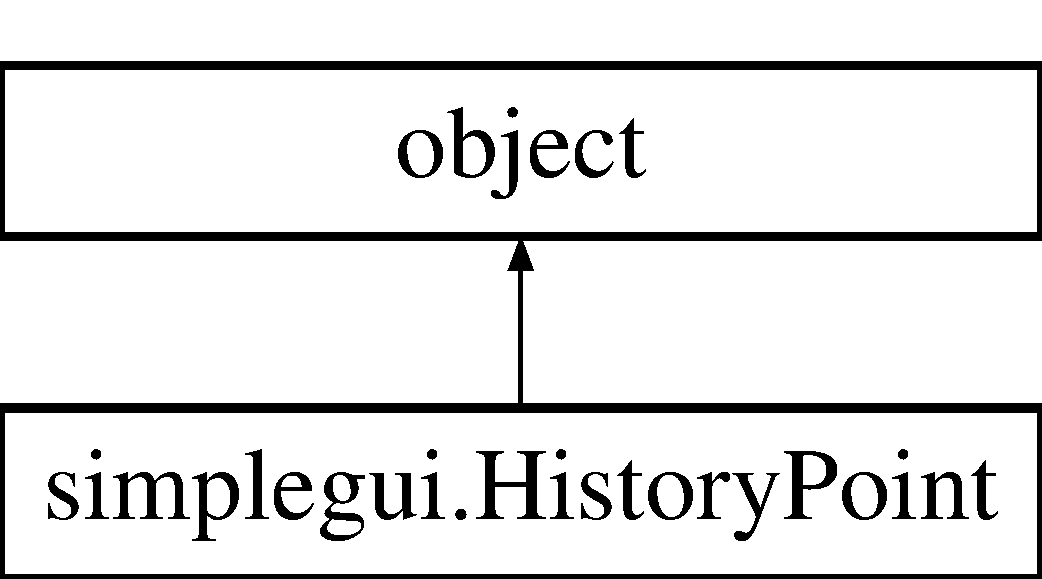
\includegraphics[height=2.000000cm]{classsimplegui_1_1_history_point}
\end{center}
\end{figure}
\subsection*{Public Member Functions}
\begin{DoxyCompactItemize}
\item 
\hypertarget{classsimplegui_1_1_history_point_adef3ead0b78d571c80b2af41a518f6c9}{def {\bfseries \-\_\-\-\_\-init\-\_\-\-\_\-}}\label{classsimplegui_1_1_history_point_adef3ead0b78d571c80b2af41a518f6c9}

\item 
\hypertarget{classsimplegui_1_1_history_point_abcec6fb63958f3afe1d5d6a389f87da2}{def {\bfseries \-\_\-\-\_\-str\-\_\-\-\_\-}}\label{classsimplegui_1_1_history_point_abcec6fb63958f3afe1d5d6a389f87da2}

\end{DoxyCompactItemize}
\subsection*{Public Attributes}
\begin{DoxyCompactItemize}
\item 
\hypertarget{classsimplegui_1_1_history_point_a0f5b051672c1140339c311a58476e912}{{\bfseries mt}}\label{classsimplegui_1_1_history_point_a0f5b051672c1140339c311a58476e912}

\item 
\hypertarget{classsimplegui_1_1_history_point_add6d6ab7f5a88db24d7ee292fa45bf86}{{\bfseries mb}}\label{classsimplegui_1_1_history_point_add6d6ab7f5a88db24d7ee292fa45bf86}

\end{DoxyCompactItemize}


\subsection{Detailed Description}
This marks a point in history. 

mt is middle top. mb is middle bottom. Because we only track middle column, ignore everything else. 

The documentation for this class was generated from the following file\-:\begin{DoxyCompactItemize}
\item 
simplegui.\-py\end{DoxyCompactItemize}

\hypertarget{classsimplegui2_1_1_history_point}{\section{simplegui2.\-History\-Point Class Reference}
\label{classsimplegui2_1_1_history_point}\index{simplegui2.\-History\-Point@{simplegui2.\-History\-Point}}
}
Inheritance diagram for simplegui2.\-History\-Point\-:\begin{figure}[H]
\begin{center}
\leavevmode
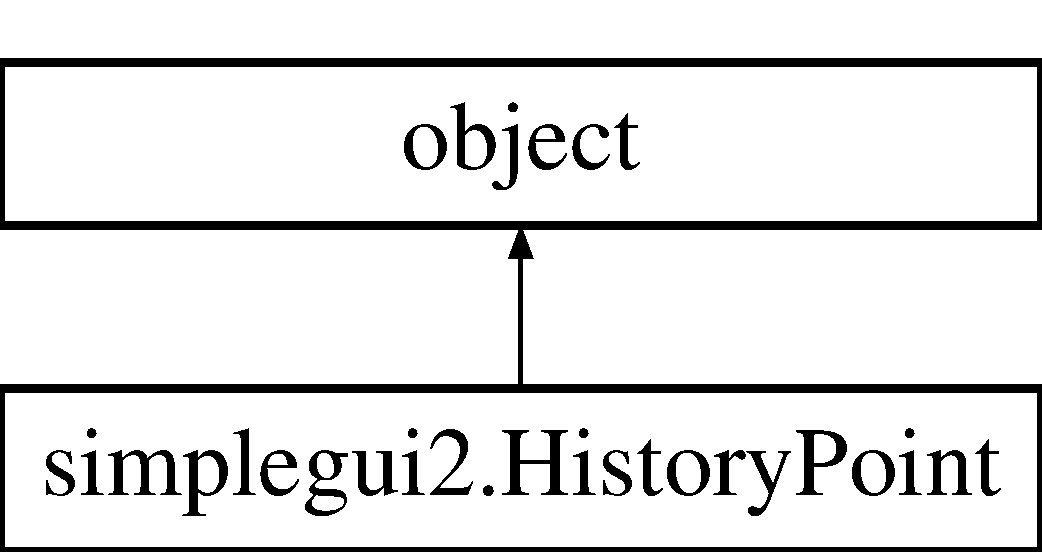
\includegraphics[height=2.000000cm]{classsimplegui2_1_1_history_point}
\end{center}
\end{figure}
\subsection*{Public Member Functions}
\begin{DoxyCompactItemize}
\item 
\hypertarget{classsimplegui2_1_1_history_point_a3a946749d474e664be06040193f33a18}{def {\bfseries \-\_\-\-\_\-init\-\_\-\-\_\-}}\label{classsimplegui2_1_1_history_point_a3a946749d474e664be06040193f33a18}

\item 
\hypertarget{classsimplegui2_1_1_history_point_accbb7614a5525ad63f09cb913fee6896}{def {\bfseries \-\_\-\-\_\-str\-\_\-\-\_\-}}\label{classsimplegui2_1_1_history_point_accbb7614a5525ad63f09cb913fee6896}

\end{DoxyCompactItemize}
\subsection*{Public Attributes}
\begin{DoxyCompactItemize}
\item 
\hypertarget{classsimplegui2_1_1_history_point_aa9b4911507b7e9d44d0c976b1a875d78}{{\bfseries mt}}\label{classsimplegui2_1_1_history_point_aa9b4911507b7e9d44d0c976b1a875d78}

\item 
\hypertarget{classsimplegui2_1_1_history_point_a56b41cda3cf4030a2ebfea5fccb9cb6d}{{\bfseries mb}}\label{classsimplegui2_1_1_history_point_a56b41cda3cf4030a2ebfea5fccb9cb6d}

\end{DoxyCompactItemize}


The documentation for this class was generated from the following file\-:\begin{DoxyCompactItemize}
\item 
simplegui2.\-py\end{DoxyCompactItemize}

\hypertarget{classsimplegui3_1_1_main_scene}{\section{simplegui3.\-Main\-Scene Class Reference}
\label{classsimplegui3_1_1_main_scene}\index{simplegui3.\-Main\-Scene@{simplegui3.\-Main\-Scene}}
}
Inheritance diagram for simplegui3.\-Main\-Scene\-:\begin{figure}[H]
\begin{center}
\leavevmode
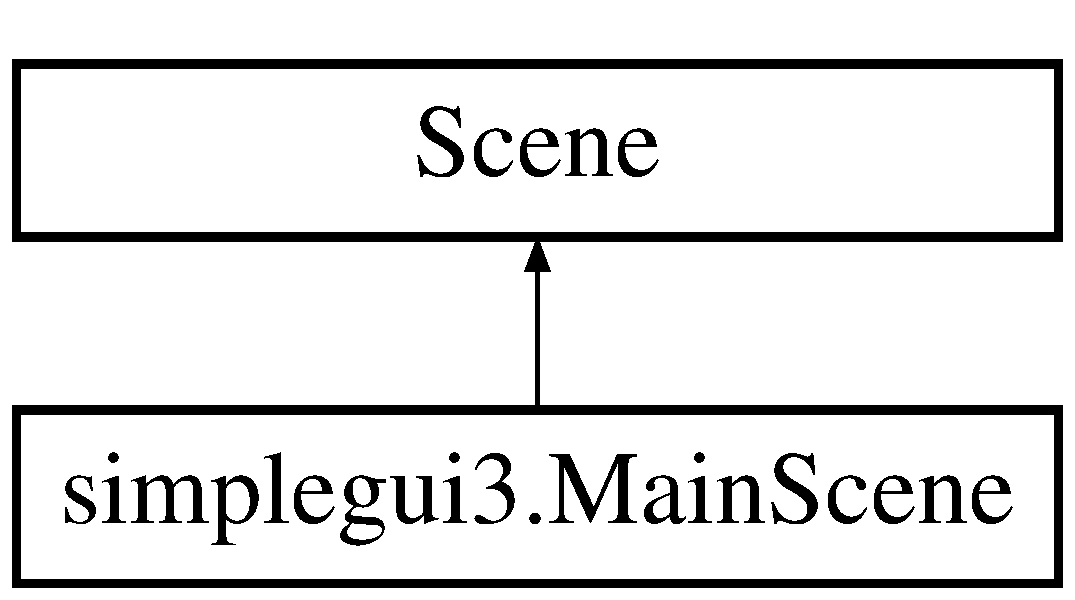
\includegraphics[height=2.000000cm]{classsimplegui3_1_1_main_scene}
\end{center}
\end{figure}
\subsection*{Public Member Functions}
\begin{DoxyCompactItemize}
\item 
\hypertarget{classsimplegui3_1_1_main_scene_aafb3c51f43351c02447d17c4e8c1fe6d}{def {\bfseries convert\-States}}\label{classsimplegui3_1_1_main_scene_aafb3c51f43351c02447d17c4e8c1fe6d}

\item 
\hypertarget{classsimplegui3_1_1_main_scene_ad09e8a3fe52fa195f7d35ddc0f101056}{def {\bfseries edit\-S\-Box}}\label{classsimplegui3_1_1_main_scene_ad09e8a3fe52fa195f7d35ddc0f101056}

\item 
\hypertarget{classsimplegui3_1_1_main_scene_a59b6e7ba6cf886c977bf5795cf72099c}{def {\bfseries run\-Round\-Keys}}\label{classsimplegui3_1_1_main_scene_a59b6e7ba6cf886c977bf5795cf72099c}

\item 
\hypertarget{classsimplegui3_1_1_main_scene_a2b683152734a69a8a09940400a5e2f11}{def {\bfseries run\-Sub\-Bytes}}\label{classsimplegui3_1_1_main_scene_a2b683152734a69a8a09940400a5e2f11}

\item 
\hypertarget{classsimplegui3_1_1_main_scene_aae7b9108cc0710126d9fd648616ef8e2}{def {\bfseries run\-Shift\-Rows}}\label{classsimplegui3_1_1_main_scene_aae7b9108cc0710126d9fd648616ef8e2}

\item 
\hypertarget{classsimplegui3_1_1_main_scene_a48b2418e3c6136be18a58c280b04a287}{def {\bfseries run\-Mix\-Columns}}\label{classsimplegui3_1_1_main_scene_a48b2418e3c6136be18a58c280b04a287}

\item 
\hypertarget{classsimplegui3_1_1_main_scene_a06d8b7a89ef09ec702d52479f8749a0f}{def {\bfseries run\-Round}}\label{classsimplegui3_1_1_main_scene_a06d8b7a89ef09ec702d52479f8749a0f}

\item 
\hypertarget{classsimplegui3_1_1_main_scene_ac0c86b509849101d4986016d670ec864}{def {\bfseries switch\-Key\-Plaintext\-Mode}}\label{classsimplegui3_1_1_main_scene_ac0c86b509849101d4986016d670ec864}

\item 
\hypertarget{classsimplegui3_1_1_main_scene_a5df983af1c795633095e0819a6360a9b}{def {\bfseries show\-Entropy}}\label{classsimplegui3_1_1_main_scene_a5df983af1c795633095e0819a6360a9b}

\item 
\hypertarget{classsimplegui3_1_1_main_scene_a939589d204d33683355ae451020fb17a}{def {\bfseries on\-Button\-Click}}\label{classsimplegui3_1_1_main_scene_a939589d204d33683355ae451020fb17a}

\item 
def \hyperlink{classsimplegui3_1_1_main_scene_ae2c8678b436ddc96acfca13a583ac51c}{update\-View}
\item 
\hypertarget{classsimplegui3_1_1_main_scene_a332ca3a94ad9e8b1f5f79ebfa42b20c1}{def {\bfseries histogram\-On\-View}}\label{classsimplegui3_1_1_main_scene_a332ca3a94ad9e8b1f5f79ebfa42b20c1}

\item 
\hypertarget{classsimplegui3_1_1_main_scene_a1fe6e0f9fc428007fb915bb635892794}{def {\bfseries punch\-Card\-On\-View}}\label{classsimplegui3_1_1_main_scene_a1fe6e0f9fc428007fb915bb635892794}

\item 
\hypertarget{classsimplegui3_1_1_main_scene_a73fd3a40a4b3776f7086ae3578aa4912}{def {\bfseries bit\-Change\-On\-View}}\label{classsimplegui3_1_1_main_scene_a73fd3a40a4b3776f7086ae3578aa4912}

\item 
\hypertarget{classsimplegui3_1_1_main_scene_a6d629320acceaed1c23ecb367f7517ff}{def {\bfseries update\-Middle\-Column}}\label{classsimplegui3_1_1_main_scene_a6d629320acceaed1c23ecb367f7517ff}

\item 
def \hyperlink{classsimplegui3_1_1_main_scene_a874aa9c53fe8eb4c5bbe2e195061b9e9}{update\-Left\-Column}
\item 
def \hyperlink{classsimplegui3_1_1_main_scene_adc63cce016c10b1c621fe9fc344661f9}{update\-Right\-Column}
\item 
def \hyperlink{classsimplegui3_1_1_main_scene_a8add894053231a29713da9e9e9671ba5}{update\-Columns}
\item 
def \hyperlink{classsimplegui3_1_1_main_scene_a4001c25db14f10aa5a32e43d20007abf}{on\-Text\-Changed}
\item 
\hypertarget{classsimplegui3_1_1_main_scene_a46f9a68956eddca314679c73f09d5a8a}{def {\bfseries moo\-\_\-changed}}\label{classsimplegui3_1_1_main_scene_a46f9a68956eddca314679c73f09d5a8a}

\item 
\hypertarget{classsimplegui3_1_1_main_scene_a706ee96ede23a5fd0d02f4faed32a350}{def {\bfseries round\-\_\-number\-\_\-changed}}\label{classsimplegui3_1_1_main_scene_a706ee96ede23a5fd0d02f4faed32a350}

\item 
\hypertarget{classsimplegui3_1_1_main_scene_af45c565c12f85f4b44e00c92d4ee56f2}{def {\bfseries expanded\-\_\-key\-\_\-size\-\_\-changed}}\label{classsimplegui3_1_1_main_scene_af45c565c12f85f4b44e00c92d4ee56f2}

\item 
\hypertarget{classsimplegui3_1_1_main_scene_a27118da38ec84d6460def7c7f805b455}{def {\bfseries visualization\-\_\-changed}}\label{classsimplegui3_1_1_main_scene_a27118da38ec84d6460def7c7f805b455}

\item 
\hypertarget{classsimplegui3_1_1_main_scene_a557ff343b6da3b25b7a98d0cf6ac1989}{def {\bfseries draw\-Top\-Bar}}\label{classsimplegui3_1_1_main_scene_a557ff343b6da3b25b7a98d0cf6ac1989}

\item 
\hypertarget{classsimplegui3_1_1_main_scene_ac8751f148908c60997904849d6d9ae0c}{def {\bfseries draw\-Bottom\-Bar}}\label{classsimplegui3_1_1_main_scene_ac8751f148908c60997904849d6d9ae0c}

\item 
def \hyperlink{classsimplegui3_1_1_main_scene_a7ee9f75298d0d2f799e6b40a71da1314}{draw\-Lines\-For\-Grid}
\item 
\hypertarget{classsimplegui3_1_1_main_scene_ab3cc10ca163c6d5eb2291e294489d151}{def {\bfseries load\-\_\-image}}\label{classsimplegui3_1_1_main_scene_ab3cc10ca163c6d5eb2291e294489d151}

\item 
def \hyperlink{classsimplegui3_1_1_main_scene_a7c4ec24817f2367e0589c74d4ab56285}{draw\-Left\-Column}
\item 
def \hyperlink{classsimplegui3_1_1_main_scene_ac2bf2c0693eadedb1207db65bb45941b}{draw\-Right\-Column}
\item 
def \hyperlink{classsimplegui3_1_1_main_scene_a6e88db4ebefebe6ade1f6267ace2c432}{draw\-Center\-Column}
\item 
\hypertarget{classsimplegui3_1_1_main_scene_aa9bda1797a7ab4d51b637174256f4e45}{def {\bfseries history\-Forward}}\label{classsimplegui3_1_1_main_scene_aa9bda1797a7ab4d51b637174256f4e45}

\item 
\hypertarget{classsimplegui3_1_1_main_scene_a3d1702ee15c64c9e9095fd241a645843}{def {\bfseries history\-Backward}}\label{classsimplegui3_1_1_main_scene_a3d1702ee15c64c9e9095fd241a645843}

\item 
\hypertarget{classsimplegui3_1_1_main_scene_ac71606a94b71c9ffcada17240752839c}{def {\bfseries print\-History}}\label{classsimplegui3_1_1_main_scene_ac71606a94b71c9ffcada17240752839c}

\item 
\hypertarget{classsimplegui3_1_1_main_scene_a90fa713384986fb426e4d86e029b2baf}{def {\bfseries add\-Point\-In\-History}}\label{classsimplegui3_1_1_main_scene_a90fa713384986fb426e4d86e029b2baf}

\item 
\hypertarget{classsimplegui3_1_1_main_scene_a22345aa823baeb2c2d50afab77665ebe}{def {\bfseries clear\-History}}\label{classsimplegui3_1_1_main_scene_a22345aa823baeb2c2d50afab77665ebe}

\item 
\hypertarget{classsimplegui3_1_1_main_scene_a1221eefea7bf8f4c4b30a4a715936f69}{def {\bfseries \-\_\-\-\_\-init\-\_\-\-\_\-}}\label{classsimplegui3_1_1_main_scene_a1221eefea7bf8f4c4b30a4a715936f69}

\item 
\hypertarget{classsimplegui3_1_1_main_scene_a23905051f31507f77786b7c9ece3a935}{def {\bfseries layout}}\label{classsimplegui3_1_1_main_scene_a23905051f31507f77786b7c9ece3a935}

\item 
\hypertarget{classsimplegui3_1_1_main_scene_ad05cc0ef1fee41a79e286e72bb738eef}{def {\bfseries update}}\label{classsimplegui3_1_1_main_scene_ad05cc0ef1fee41a79e286e72bb738eef}

\item 
\hypertarget{classsimplegui3_1_1_main_scene_ac95a24af359c8d462d85c02de695dc30}{def {\bfseries get\-R\-G\-B}}\label{classsimplegui3_1_1_main_scene_ac95a24af359c8d462d85c02de695dc30}

\end{DoxyCompactItemize}
\subsection*{Public Attributes}
\begin{DoxyCompactItemize}
\item 
\hypertarget{classsimplegui3_1_1_main_scene_a39da922b65d26fd408d5a348b9bfa504}{{\bfseries ptk\-Mode}}\label{classsimplegui3_1_1_main_scene_a39da922b65d26fd408d5a348b9bfa504}

\item 
\hypertarget{classsimplegui3_1_1_main_scene_a712a5214570815763f1eaa732ecef5f6}{{\bfseries lb\-Entry}}\label{classsimplegui3_1_1_main_scene_a712a5214570815763f1eaa732ecef5f6}

\item 
\hypertarget{classsimplegui3_1_1_main_scene_a5483f2561f1b9f6f4e37367fa60f5c0d}{{\bfseries lt\-Entry}}\label{classsimplegui3_1_1_main_scene_a5483f2561f1b9f6f4e37367fa60f5c0d}

\item 
\hypertarget{classsimplegui3_1_1_main_scene_aae9768d78d612c39c585066c5fb39465}{{\bfseries lm\-Entry}}\label{classsimplegui3_1_1_main_scene_aae9768d78d612c39c585066c5fb39465}

\item 
\hypertarget{classsimplegui3_1_1_main_scene_a71679de64801b99cfa87bc0bc88ac6e0}{{\bfseries original\-Entropy}}\label{classsimplegui3_1_1_main_scene_a71679de64801b99cfa87bc0bc88ac6e0}

\item 
\hypertarget{classsimplegui3_1_1_main_scene_ad37b8d779897b143cc284206ed55f6ac}{{\bfseries states\-Entropy}}\label{classsimplegui3_1_1_main_scene_ad37b8d779897b143cc284206ed55f6ac}

\item 
\hypertarget{classsimplegui3_1_1_main_scene_a82c3188b5645b3b3f11d5bf7408dfda2}{{\bfseries crypts\-Entropy}}\label{classsimplegui3_1_1_main_scene_a82c3188b5645b3b3f11d5bf7408dfda2}

\item 
\hypertarget{classsimplegui3_1_1_main_scene_a9f16b024bd3f0563146d604250c66986}{{\bfseries cleartext}}\label{classsimplegui3_1_1_main_scene_a9f16b024bd3f0563146d604250c66986}

\item 
\hypertarget{classsimplegui3_1_1_main_scene_a970a21b91cbe1f94a44f70c8c4aae6f8}{{\bfseries visualization}}\label{classsimplegui3_1_1_main_scene_a970a21b91cbe1f94a44f70c8c4aae6f8}

\item 
\hypertarget{classsimplegui3_1_1_main_scene_adfc2426d6b446729496113eceb734692}{{\bfseries operation\-Mode}}\label{classsimplegui3_1_1_main_scene_adfc2426d6b446729496113eceb734692}

\item 
\hypertarget{classsimplegui3_1_1_main_scene_a8ab3c9afb69754b4ede968584877f8b3}{{\bfseries key\-Size}}\label{classsimplegui3_1_1_main_scene_a8ab3c9afb69754b4ede968584877f8b3}

\item 
\hypertarget{classsimplegui3_1_1_main_scene_ac9a8ccc9dd35fc75f4ea8e6d89d4dfb2}{{\bfseries plaintextone\-\_\-imageview}}\label{classsimplegui3_1_1_main_scene_ac9a8ccc9dd35fc75f4ea8e6d89d4dfb2}

\item 
\hypertarget{classsimplegui3_1_1_main_scene_aad2c95da342b2028821655c2e99a0b2f}{{\bfseries plaintexttwo\-\_\-imageview}}\label{classsimplegui3_1_1_main_scene_aad2c95da342b2028821655c2e99a0b2f}

\item 
\hypertarget{classsimplegui3_1_1_main_scene_ae5bc536c0d0b6ca74de421af036305d0}{{\bfseries lefttop\-\_\-textfield}}\label{classsimplegui3_1_1_main_scene_ae5bc536c0d0b6ca74de421af036305d0}

\item 
\hypertarget{classsimplegui3_1_1_main_scene_ad1dded208f7978a1073bd6dca5284b2b}{{\bfseries leftbottom\-\_\-textfield}}\label{classsimplegui3_1_1_main_scene_ad1dded208f7978a1073bd6dca5284b2b}

\item 
\hypertarget{classsimplegui3_1_1_main_scene_a7cfae13ce52eb3249f52e4c0d16121d2}{{\bfseries leftmiddle\-\_\-textfield}}\label{classsimplegui3_1_1_main_scene_a7cfae13ce52eb3249f52e4c0d16121d2}

\item 
\hypertarget{classsimplegui3_1_1_main_scene_a883a37f7c8e05945f50c15d98be68807}{{\bfseries cipherone\-\_\-imageview}}\label{classsimplegui3_1_1_main_scene_a883a37f7c8e05945f50c15d98be68807}

\item 
\hypertarget{classsimplegui3_1_1_main_scene_a52cfa25ba7e5e295e5cd81ae7f2bb263}{{\bfseries ciphertwo\-\_\-imageview}}\label{classsimplegui3_1_1_main_scene_a52cfa25ba7e5e295e5cd81ae7f2bb263}

\item 
\hypertarget{classsimplegui3_1_1_main_scene_a6732bbc18043c30bb2c07fd4d747d25a}{{\bfseries currentone\-\_\-imageview}}\label{classsimplegui3_1_1_main_scene_a6732bbc18043c30bb2c07fd4d747d25a}

\item 
\hypertarget{classsimplegui3_1_1_main_scene_a896c069c7fcfbee557c432c51d29d144}{{\bfseries currenttwo\-\_\-imageview}}\label{classsimplegui3_1_1_main_scene_a896c069c7fcfbee557c432c51d29d144}

\item 
\hypertarget{classsimplegui3_1_1_main_scene_aa01e5f4ac65a2a9ca7cda315e39867d1}{{\bfseries future}}\label{classsimplegui3_1_1_main_scene_aa01e5f4ac65a2a9ca7cda315e39867d1}

\item 
\hypertarget{classsimplegui3_1_1_main_scene_a15824a98b4468c93364e4a1a891d98ee}{{\bfseries history}}\label{classsimplegui3_1_1_main_scene_a15824a98b4468c93364e4a1a891d98ee}

\item 
\hypertarget{classsimplegui3_1_1_main_scene_a52ee56cfa161887c384a6ef6c825c1ef}{{\bfseries moo}}\label{classsimplegui3_1_1_main_scene_a52ee56cfa161887c384a6ef6c825c1ef}

\item 
\hypertarget{classsimplegui3_1_1_main_scene_a4d842426a675e1e48626af56e9e0cc58}{{\bfseries cypherkey}}\label{classsimplegui3_1_1_main_scene_a4d842426a675e1e48626af56e9e0cc58}

\item 
\hypertarget{classsimplegui3_1_1_main_scene_aefa8a89f9b0fcc59b2215f4793fb4ef1}{{\bfseries iv}}\label{classsimplegui3_1_1_main_scene_aefa8a89f9b0fcc59b2215f4793fb4ef1}

\item 
\hypertarget{classsimplegui3_1_1_main_scene_a49c2fd5260ea208f24022cbd5a2b6e5b}{{\bfseries label\-\_\-height}}\label{classsimplegui3_1_1_main_scene_a49c2fd5260ea208f24022cbd5a2b6e5b}

\item 
\hypertarget{classsimplegui3_1_1_main_scene_a6e44e3320fee1c94f4392fa3b2db534a}{{\bfseries button\-Bar\-Bottom}}\label{classsimplegui3_1_1_main_scene_a6e44e3320fee1c94f4392fa3b2db534a}

\item 
\hypertarget{classsimplegui3_1_1_main_scene_ab214ae8cd678f27ff6557b109c471585}{{\bfseries column\-Width}}\label{classsimplegui3_1_1_main_scene_ab214ae8cd678f27ff6557b109c471585}

\item 
\hypertarget{classsimplegui3_1_1_main_scene_a8b54bf8731d97bdeda46f4a5e99b392c}{{\bfseries middle\-Bar\-Y}}\label{classsimplegui3_1_1_main_scene_a8b54bf8731d97bdeda46f4a5e99b392c}

\item 
\hypertarget{classsimplegui3_1_1_main_scene_a9bd255b2be318bb2a79207085cf78173}{{\bfseries empty}}\label{classsimplegui3_1_1_main_scene_a9bd255b2be318bb2a79207085cf78173}

\end{DoxyCompactItemize}
\subsection*{Static Public Attributes}
\begin{DoxyCompactItemize}
\item 
\hypertarget{classsimplegui3_1_1_main_scene_a78e2027ae1ef8d98bfa58dd6737373a2}{tuple {\bfseries aes} = \hyperlink{classslowaes_1_1_a_e_s}{slowaes.\-A\-E\-S}()}\label{classsimplegui3_1_1_main_scene_a78e2027ae1ef8d98bfa58dd6737373a2}

\item 
\hypertarget{classsimplegui3_1_1_main_scene_a980ca4a42256d9f2551b999521a54ab5}{tuple {\bfseries aesmoo} = \hyperlink{classslowaes_1_1_a_e_s_mode_of_operation}{slowaes.\-A\-E\-S\-Mode\-Of\-Operation}()}\label{classsimplegui3_1_1_main_scene_a980ca4a42256d9f2551b999521a54ab5}

\end{DoxyCompactItemize}


\subsection{Member Function Documentation}
\hypertarget{classsimplegui3_1_1_main_scene_a6e88db4ebefebe6ade1f6267ace2c432}{\index{simplegui3\-::\-Main\-Scene@{simplegui3\-::\-Main\-Scene}!draw\-Center\-Column@{draw\-Center\-Column}}
\index{draw\-Center\-Column@{draw\-Center\-Column}!simplegui3::MainScene@{simplegui3\-::\-Main\-Scene}}
\subsubsection[{draw\-Center\-Column}]{\setlength{\rightskip}{0pt plus 5cm}def simplegui3.\-Main\-Scene.\-draw\-Center\-Column (
\begin{DoxyParamCaption}
\item[{}]{self}
\end{DoxyParamCaption}
)}}\label{classsimplegui3_1_1_main_scene_a6e88db4ebefebe6ade1f6267ace2c432}
\begin{DoxyVerb}    This draws the center column.
    This will be the current cipher keys and a slider at the bottom
    for history.
\end{DoxyVerb}
 \hypertarget{classsimplegui3_1_1_main_scene_a7c4ec24817f2367e0589c74d4ab56285}{\index{simplegui3\-::\-Main\-Scene@{simplegui3\-::\-Main\-Scene}!draw\-Left\-Column@{draw\-Left\-Column}}
\index{draw\-Left\-Column@{draw\-Left\-Column}!simplegui3::MainScene@{simplegui3\-::\-Main\-Scene}}
\subsubsection[{draw\-Left\-Column}]{\setlength{\rightskip}{0pt plus 5cm}def simplegui3.\-Main\-Scene.\-draw\-Left\-Column (
\begin{DoxyParamCaption}
\item[{}]{self}
\end{DoxyParamCaption}
)}}\label{classsimplegui3_1_1_main_scene_a7c4ec24817f2367e0589c74d4ab56285}
\begin{DoxyVerb}    This draws the left column.
    This column consists of two surfaces showing the initial string,
    along input text boxes for the strings.
\end{DoxyVerb}
 \hypertarget{classsimplegui3_1_1_main_scene_a7ee9f75298d0d2f799e6b40a71da1314}{\index{simplegui3\-::\-Main\-Scene@{simplegui3\-::\-Main\-Scene}!draw\-Lines\-For\-Grid@{draw\-Lines\-For\-Grid}}
\index{draw\-Lines\-For\-Grid@{draw\-Lines\-For\-Grid}!simplegui3::MainScene@{simplegui3\-::\-Main\-Scene}}
\subsubsection[{draw\-Lines\-For\-Grid}]{\setlength{\rightskip}{0pt plus 5cm}def simplegui3.\-Main\-Scene.\-draw\-Lines\-For\-Grid (
\begin{DoxyParamCaption}
\item[{}]{self}
\end{DoxyParamCaption}
)}}\label{classsimplegui3_1_1_main_scene_a7ee9f75298d0d2f799e6b40a71da1314}
\begin{DoxyVerb}    This draws the grid lines.
    This includes the two lines going top to bottom for each column.
    This also includes the bar below the buttons at the top and the
    middle horizontal line separating the two plain texts, cipher texts
    and current progress.
\end{DoxyVerb}
 \hypertarget{classsimplegui3_1_1_main_scene_ac2bf2c0693eadedb1207db65bb45941b}{\index{simplegui3\-::\-Main\-Scene@{simplegui3\-::\-Main\-Scene}!draw\-Right\-Column@{draw\-Right\-Column}}
\index{draw\-Right\-Column@{draw\-Right\-Column}!simplegui3::MainScene@{simplegui3\-::\-Main\-Scene}}
\subsubsection[{draw\-Right\-Column}]{\setlength{\rightskip}{0pt plus 5cm}def simplegui3.\-Main\-Scene.\-draw\-Right\-Column (
\begin{DoxyParamCaption}
\item[{}]{self}
\end{DoxyParamCaption}
)}}\label{classsimplegui3_1_1_main_scene_ac2bf2c0693eadedb1207db65bb45941b}
\begin{DoxyVerb}    This draws the right column.
    This will be the normal result of the plain texts if ran normally
    through AES.
\end{DoxyVerb}
 \hypertarget{classsimplegui3_1_1_main_scene_a4001c25db14f10aa5a32e43d20007abf}{\index{simplegui3\-::\-Main\-Scene@{simplegui3\-::\-Main\-Scene}!on\-Text\-Changed@{on\-Text\-Changed}}
\index{on\-Text\-Changed@{on\-Text\-Changed}!simplegui3::MainScene@{simplegui3\-::\-Main\-Scene}}
\subsubsection[{on\-Text\-Changed}]{\setlength{\rightskip}{0pt plus 5cm}def simplegui3.\-Main\-Scene.\-on\-Text\-Changed (
\begin{DoxyParamCaption}
\item[{}]{self, }
\item[{}]{tf, }
\item[{}]{text}
\end{DoxyParamCaption}
)}}\label{classsimplegui3_1_1_main_scene_a4001c25db14f10aa5a32e43d20007abf}
\begin{DoxyVerb}tf is the TextField object.
    Text is the text the TextField was changed to.
\end{DoxyVerb}
 \hypertarget{classsimplegui3_1_1_main_scene_a8add894053231a29713da9e9e9671ba5}{\index{simplegui3\-::\-Main\-Scene@{simplegui3\-::\-Main\-Scene}!update\-Columns@{update\-Columns}}
\index{update\-Columns@{update\-Columns}!simplegui3::MainScene@{simplegui3\-::\-Main\-Scene}}
\subsubsection[{update\-Columns}]{\setlength{\rightskip}{0pt plus 5cm}def simplegui3.\-Main\-Scene.\-update\-Columns (
\begin{DoxyParamCaption}
\item[{}]{self}
\end{DoxyParamCaption}
)}}\label{classsimplegui3_1_1_main_scene_a8add894053231a29713da9e9e9671ba5}
\begin{DoxyVerb}This updates all the columns.  Redraws the left, right, and center. \end{DoxyVerb}
 \hypertarget{classsimplegui3_1_1_main_scene_a874aa9c53fe8eb4c5bbe2e195061b9e9}{\index{simplegui3\-::\-Main\-Scene@{simplegui3\-::\-Main\-Scene}!update\-Left\-Column@{update\-Left\-Column}}
\index{update\-Left\-Column@{update\-Left\-Column}!simplegui3::MainScene@{simplegui3\-::\-Main\-Scene}}
\subsubsection[{update\-Left\-Column}]{\setlength{\rightskip}{0pt plus 5cm}def simplegui3.\-Main\-Scene.\-update\-Left\-Column (
\begin{DoxyParamCaption}
\item[{}]{self}
\end{DoxyParamCaption}
)}}\label{classsimplegui3_1_1_main_scene_a874aa9c53fe8eb4c5bbe2e195061b9e9}
\begin{DoxyVerb}This should update the left column \end{DoxyVerb}
 \hypertarget{classsimplegui3_1_1_main_scene_adc63cce016c10b1c621fe9fc344661f9}{\index{simplegui3\-::\-Main\-Scene@{simplegui3\-::\-Main\-Scene}!update\-Right\-Column@{update\-Right\-Column}}
\index{update\-Right\-Column@{update\-Right\-Column}!simplegui3::MainScene@{simplegui3\-::\-Main\-Scene}}
\subsubsection[{update\-Right\-Column}]{\setlength{\rightskip}{0pt plus 5cm}def simplegui3.\-Main\-Scene.\-update\-Right\-Column (
\begin{DoxyParamCaption}
\item[{}]{self}
\end{DoxyParamCaption}
)}}\label{classsimplegui3_1_1_main_scene_adc63cce016c10b1c621fe9fc344661f9}
\begin{DoxyVerb}This should update the right column \end{DoxyVerb}
 \hypertarget{classsimplegui3_1_1_main_scene_ae2c8678b436ddc96acfca13a583ac51c}{\index{simplegui3\-::\-Main\-Scene@{simplegui3\-::\-Main\-Scene}!update\-View@{update\-View}}
\index{update\-View@{update\-View}!simplegui3::MainScene@{simplegui3\-::\-Main\-Scene}}
\subsubsection[{update\-View}]{\setlength{\rightskip}{0pt plus 5cm}def simplegui3.\-Main\-Scene.\-update\-View (
\begin{DoxyParamCaption}
\item[{}]{self, }
\item[{}]{text, }
\item[{}]{view, }
\item[{}]{size}
\end{DoxyParamCaption}
)}}\label{classsimplegui3_1_1_main_scene_ae2c8678b436ddc96acfca13a583ac51c}
\begin{DoxyVerb}    This method accepts a string, cipher/plain text (text), and updates the view (view) given.
    The size is a tuple (#,#) that is the resulting size.
\end{DoxyVerb}
 

The documentation for this class was generated from the following file\-:\begin{DoxyCompactItemize}
\item 
simplegui3.\-py\end{DoxyCompactItemize}

\hypertarget{classsimplegui_1_1_main_scene}{\section{simplegui.\-Main\-Scene Class Reference}
\label{classsimplegui_1_1_main_scene}\index{simplegui.\-Main\-Scene@{simplegui.\-Main\-Scene}}
}


A Scene object, from the pygameui library.  


Inheritance diagram for simplegui.\-Main\-Scene\-:\begin{figure}[H]
\begin{center}
\leavevmode
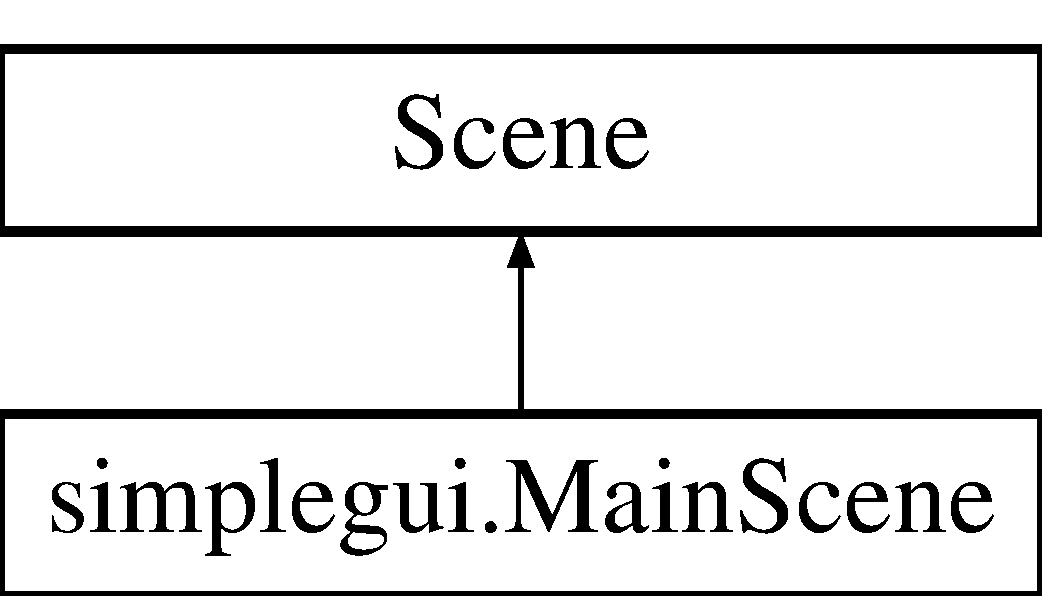
\includegraphics[height=2.000000cm]{classsimplegui_1_1_main_scene}
\end{center}
\end{figure}
\subsection*{Public Member Functions}
\begin{DoxyCompactItemize}
\item 
\hypertarget{classsimplegui_1_1_main_scene_a2c8156bf798a6cbcc85f8f70b92877c1}{def {\bfseries set\-To\-Prob\-Dist}}\label{classsimplegui_1_1_main_scene_a2c8156bf798a6cbcc85f8f70b92877c1}

\item 
def \hyperlink{classsimplegui_1_1_main_scene_ac7eb263562c3f9a992a00d43ddd7d1a6}{kl}
\begin{DoxyCompactList}\small\item\em one and two are both probability distributions for the sets. \end{DoxyCompactList}\item 
def \hyperlink{classsimplegui_1_1_main_scene_a2fedafb26922217bff2c9b4f0a1e1980}{convert\-States}
\begin{DoxyCompactList}\small\item\em Converts input to usable (With slowaes) int arrays. \end{DoxyCompactList}\item 
def \hyperlink{classsimplegui_1_1_main_scene_a464f594963c80652f89a341d86e675ab}{edit\-S\-Box}
\begin{DoxyCompactList}\small\item\em Change between the all 0s in the s box and just the normal s box. \end{DoxyCompactList}\item 
<<<<<<< HEAD
def \hyperlink{classsimplegui_1_1_main_scene_a3e84e45150794e1806472cd45904f9b9}{run\-Round}
\begin{DoxyCompactList}\small\item\em This method runs a round like normal using the 4 subroutines. \end{DoxyCompactList}\item 
def \hyperlink{classsimplegui_1_1_main_scene_a13363bc98bb9603d8c0ab35d52cc853b}{run\-Add\-Round\-Key}
=======
def \hyperlink{classsimplegui_1_1_main_scene_a6616923509a481f8ab7c99a2764ef5ec}{run\-Round\-Keys}
>>>>>>> 0f00e98e69f9936960b63973a11aea6e6dd4ee45
\begin{DoxyCompactList}\small\item\em Run the round key function on the information. \end{DoxyCompactList}\item 
def \hyperlink{classsimplegui_1_1_main_scene_a8e81494def3ea3c0e56813f6d702a435}{run\-Sub\-Bytes}
\begin{DoxyCompactList}\small\item\em Runs the sub bytes on the current values. \end{DoxyCompactList}\item 
\hypertarget{classsimplegui_1_1_main_scene_a900ce77068dfc386d298f7ef1243529a}{def \hyperlink{classsimplegui_1_1_main_scene_a900ce77068dfc386d298f7ef1243529a}{run\-Shift\-Rows}}\label{classsimplegui_1_1_main_scene_a900ce77068dfc386d298f7ef1243529a}

\begin{DoxyCompactList}\small\item\em Run shift row subroutine of A\-E\-S and updates middle column. \end{DoxyCompactList}\item 
\hypertarget{classsimplegui_1_1_main_scene_a805cca2ef3e4086eb23505b8af930f18}{def \hyperlink{classsimplegui_1_1_main_scene_a805cca2ef3e4086eb23505b8af930f18}{run\-Mix\-Columns}}\label{classsimplegui_1_1_main_scene_a805cca2ef3e4086eb23505b8af930f18}

\begin{DoxyCompactList}\small\item\em Run mix column subroutine of A\-E\-S and updates middle column. \end{DoxyCompactList}\item 
def \hyperlink{classsimplegui_1_1_main_scene_a8570c31330b924dce8f26088e4e3fa3e}{switch\-Key\-Plaintext\-Mode}
\begin{DoxyCompactList}\small\item\em Switches between 2 plain texts, 1 key and 1 plain text, 2 keys. \end{DoxyCompactList}\item 
def \hyperlink{classsimplegui_1_1_main_scene_aaeb0e4df3ab8dd5a9cab35f28ad2f7a2}{on\-Button\-Click}
\begin{DoxyCompactList}\small\item\em Ran when a button is clicked. \end{DoxyCompactList}\item 
def \hyperlink{classsimplegui_1_1_main_scene_a1e32c0468a9abbd3e0e6b418c788c4e0}{update\-View}
\begin{DoxyCompactList}\small\item\em Updates the view for greyscale and color scale types. \end{DoxyCompactList}\item 
def \hyperlink{classsimplegui_1_1_main_scene_a1104ae8cca81e51cc77524c7e048464d}{histogram\-On\-View}
\begin{DoxyCompactList}\small\item\em Creates the histogram on the surfaces. \end{DoxyCompactList}\item 
def \hyperlink{classsimplegui_1_1_main_scene_a7155c316b15f3ff406c0fa44500ba768}{bit\-Change\-On\-View}
\begin{DoxyCompactList}\small\item\em Updates the surfaces to show the bit change visualization. \end{DoxyCompactList}\item 
def \hyperlink{classsimplegui_1_1_main_scene_a22c60c1b880ee015c51e35dce45a8267}{update\-Middle\-Column}
\begin{DoxyCompactList}\small\item\em Updates the middle column. \end{DoxyCompactList}\item 
def \hyperlink{classsimplegui_1_1_main_scene_af271c4ea829421b364c9ccce3ea6d88a}{update\-Left\-Column}
\begin{DoxyCompactList}\small\item\em Updates the left column. \end{DoxyCompactList}\item 
def \hyperlink{classsimplegui_1_1_main_scene_a9feca10a8fe6385d3515407200d70789}{update\-Right\-Column}
\begin{DoxyCompactList}\small\item\em Updates the right column. \end{DoxyCompactList}\item 
def \hyperlink{classsimplegui_1_1_main_scene_a3f57128f4c0a7608e2b6514915fdb821}{update\-Columns}
\begin{DoxyCompactList}\small\item\em Easy way to update all columns. \end{DoxyCompactList}\item 
def \hyperlink{classsimplegui_1_1_main_scene_af3b0457ad0c83dbe77810352fc765904}{on\-Text\-Changed}
\begin{DoxyCompactList}\small\item\em Ran when text is changed in any of the input boxes. \end{DoxyCompactList}\item 
def \hyperlink{classsimplegui_1_1_main_scene_acfb4597c5d0766c02a140455b80ec1f3}{moo\-\_\-changed}
\begin{DoxyCompactList}\small\item\em Ran when mode of operation is changed. \end{DoxyCompactList}\item 
\hypertarget{classsimplegui_1_1_main_scene_aecc02f06c9b870a63c17099f1c683b32}{def \hyperlink{classsimplegui_1_1_main_scene_aecc02f06c9b870a63c17099f1c683b32}{round\-\_\-number\-\_\-changed}}\label{classsimplegui_1_1_main_scene_aecc02f06c9b870a63c17099f1c683b32}

\begin{DoxyCompactList}\small\item\em Ran when round number is changed (Just updates the columns) \end{DoxyCompactList}\item 
def \hyperlink{classsimplegui_1_1_main_scene_aeb4a9163209211e2da60c5956d0f0028}{expanded\-\_\-key\-\_\-size\-\_\-changed}
\begin{DoxyCompactList}\small\item\em Expanded key size (128/192/256) was changed. \end{DoxyCompactList}\item 
def \hyperlink{classsimplegui_1_1_main_scene_aa53b6cd3c1c56ced6a8fe4b98602314e}{visualization\-\_\-changed}
\begin{DoxyCompactList}\small\item\em Visualizaiton changed, update views. \end{DoxyCompactList}\item 
def \hyperlink{classsimplegui_1_1_main_scene_a46b737949a8af3c0637f63e3223c655d}{draw\-Top\-Bar}
\begin{DoxyCompactList}\small\item\em Draws the top bar U\-I elements. \end{DoxyCompactList}\item 
def \hyperlink{classsimplegui_1_1_main_scene_ab5ce2a41f55ec406f4902fb0ce2a5845}{draw\-Bottom\-Bar}
\begin{DoxyCompactList}\small\item\em Draws the bottom bar U\-I elements. \end{DoxyCompactList}\item 
def \hyperlink{classsimplegui_1_1_main_scene_ab5ba5b0e3ab5ac61668929effb1a5544}{draw\-Lines\-For\-Grid}
\begin{DoxyCompactList}\small\item\em Draws the lines separaring the bars and the columns for U\-I elements. \end{DoxyCompactList}\item 
def \hyperlink{classsimplegui_1_1_main_scene_a3a8096d9c941aacdee8e159858f67866}{load\-\_\-image}
\begin{DoxyCompactList}\small\item\em A stupid method needed to draw a surface in the columns. \end{DoxyCompactList}\item 
def \hyperlink{classsimplegui_1_1_main_scene_a74c3de5ad8f9cbf50fd626e539ec29d1}{draw\-Left\-Column}
\begin{DoxyCompactList}\small\item\em Draws the left column U\-I elements. \end{DoxyCompactList}\item 
def \hyperlink{classsimplegui_1_1_main_scene_adf07e31f3e330acfdf78ca1155e65fd0}{draw\-Right\-Column}
\begin{DoxyCompactList}\small\item\em Draws the right column U\-I elements. \end{DoxyCompactList}\item 
def \hyperlink{classsimplegui_1_1_main_scene_a17c05e23835e26489665463846367443}{draw\-Center\-Column}
\begin{DoxyCompactList}\small\item\em Draws the center column U\-I elements. \end{DoxyCompactList}\item 
def \hyperlink{classsimplegui_1_1_main_scene_a8b2f261a306a2919d702e57475f15589}{history\-Forward}
\begin{DoxyCompactList}\small\item\em Called when we're moving forward in history. \end{DoxyCompactList}\item 
def \hyperlink{classsimplegui_1_1_main_scene_ac745bb4c5e46e8abfb92619905ff9845}{history\-Backward}
\begin{DoxyCompactList}\small\item\em Called when we're moving backward in history. \end{DoxyCompactList}\item 
def \hyperlink{classsimplegui_1_1_main_scene_a85395ee516211bc07cdd7ff765158de0}{print\-History}
\begin{DoxyCompactList}\small\item\em Debug method. \end{DoxyCompactList}\item 
def \hyperlink{classsimplegui_1_1_main_scene_a8c7e504663d3819336e4df829e9819cf}{add\-Point\-In\-History}
\begin{DoxyCompactList}\small\item\em Adds a point to our history, resets the future. \end{DoxyCompactList}\item 
def \hyperlink{classsimplegui_1_1_main_scene_a2e495c8b6cf4da78947791e42dcd8f42}{clear\-History}
\begin{DoxyCompactList}\small\item\em Clears all history, or resets the history. \end{DoxyCompactList}\item 
def \hyperlink{classsimplegui_1_1_main_scene_a1771d66ba1c6fdb7f2b3c04f4173a9e3}{\-\_\-\-\_\-init\-\_\-\-\_\-}
\begin{DoxyCompactList}\small\item\em Initializes items, variables, etc. \end{DoxyCompactList}\item 
def \hyperlink{classsimplegui_1_1_main_scene_a82073a2b7ed88995f266a06b7f9ec6be}{layout}
\begin{DoxyCompactList}\small\item\em Used by the pygameui library. \end{DoxyCompactList}\item 
def \hyperlink{classsimplegui_1_1_main_scene_abe88eb59c38cba1d558fb8bcc672e929}{update}
\begin{DoxyCompactList}\small\item\em Used by the pygameui library. \end{DoxyCompactList}\item 
def \hyperlink{classsimplegui_1_1_main_scene_a68319a096ea4237e209e861005e1aaf7}{get\-R\-G\-B}
\begin{DoxyCompactList}\small\item\em Helper method to get color values (R\-G\-B) from an 8 bit number. \end{DoxyCompactList}\end{DoxyCompactItemize}
\subsection*{Public Attributes}
\begin{DoxyCompactItemize}
\item 
\hypertarget{classsimplegui_1_1_main_scene_a3caeb0ed63f79e39b6cb371333588459}{{\bfseries lrb\-Entry}}\label{classsimplegui_1_1_main_scene_a3caeb0ed63f79e39b6cb371333588459}

\item 
<<<<<<< HEAD
\hypertarget{classsimplegui_1_1_main_scene_a397b09a55f332b362aa9ed4a4cc93888}{{\bfseries lrt\-Entry}}\label{classsimplegui_1_1_main_scene_a397b09a55f332b362aa9ed4a4cc93888}

\item 
=======
>>>>>>> 0f00e98e69f9936960b63973a11aea6e6dd4ee45
\hypertarget{classsimplegui_1_1_main_scene_a6f6b3ee72b43ee95448828b8dd1fe675}{{\bfseries ptk\-Mode}}\label{classsimplegui_1_1_main_scene_a6f6b3ee72b43ee95448828b8dd1fe675}

\item 
\hypertarget{classsimplegui_1_1_main_scene_a5dd2dd757387dfd57519b395382b23d2}{{\bfseries llb\-Entry}}\label{classsimplegui_1_1_main_scene_a5dd2dd757387dfd57519b395382b23d2}

\item 
\hypertarget{classsimplegui_1_1_main_scene_af83011177cccee7fd54e54be752e0a58}{{\bfseries llt\-Entry}}\label{classsimplegui_1_1_main_scene_af83011177cccee7fd54e54be752e0a58}

\item 
<<<<<<< HEAD
\hypertarget{classsimplegui_1_1_main_scene_a12caf5854924dac329f3ee95d5c2f67f}{{\bfseries old\-S\-Box}}\label{classsimplegui_1_1_main_scene_a12caf5854924dac329f3ee95d5c2f67f}

\item 
\hypertarget{classsimplegui_1_1_main_scene_ab5c6e082bdf28d47e18c15115fb9d29a}{{\bfseries old\-R\-S\-Box}}\label{classsimplegui_1_1_main_scene_ab5c6e082bdf28d47e18c15115fb9d29a}

\item 
\hypertarget{classsimplegui_1_1_main_scene_a07365b93310d51583324117e96f548c7}{{\bfseries key\-Size}}\label{classsimplegui_1_1_main_scene_a07365b93310d51583324117e96f548c7}
=======
\hypertarget{classsimplegui_1_1_main_scene_a397b09a55f332b362aa9ed4a4cc93888}{{\bfseries lrt\-Entry}}\label{classsimplegui_1_1_main_scene_a397b09a55f332b362aa9ed4a4cc93888}

\item 
\hypertarget{classsimplegui_1_1_main_scene_a12caf5854924dac329f3ee95d5c2f67f}{{\bfseries old\-S\-Box}}\label{classsimplegui_1_1_main_scene_a12caf5854924dac329f3ee95d5c2f67f}

\item 
\hypertarget{classsimplegui_1_1_main_scene_ab5c6e082bdf28d47e18c15115fb9d29a}{{\bfseries old\-R\-S\-Box}}\label{classsimplegui_1_1_main_scene_ab5c6e082bdf28d47e18c15115fb9d29a}
>>>>>>> 0f00e98e69f9936960b63973a11aea6e6dd4ee45

\item 
\hypertarget{classsimplegui_1_1_main_scene_ae295a66ef3135a9f1f445a82d8b4d647}{{\bfseries cleartext}}\label{classsimplegui_1_1_main_scene_ae295a66ef3135a9f1f445a82d8b4d647}

\item 
\hypertarget{classsimplegui_1_1_main_scene_a2522d257feb552ec87215e4af1055852}{{\bfseries visualization}}\label{classsimplegui_1_1_main_scene_a2522d257feb552ec87215e4af1055852}

\item 
\hypertarget{classsimplegui_1_1_main_scene_ab5d4615ae42d5c705ba4398b3e33fc7a}{{\bfseries cypherkey}}\label{classsimplegui_1_1_main_scene_ab5d4615ae42d5c705ba4398b3e33fc7a}

\item 
\hypertarget{classsimplegui_1_1_main_scene_aac7f93fc2da16c5425f60138e3b1ce51}{{\bfseries operation\-Mode}}\label{classsimplegui_1_1_main_scene_aac7f93fc2da16c5425f60138e3b1ce51}

\item 
<<<<<<< HEAD
\hypertarget{classsimplegui_1_1_main_scene_a1e40227d207ff4128178318f46b7eb64}{{\bfseries cur\-Round}}\label{classsimplegui_1_1_main_scene_a1e40227d207ff4128178318f46b7eb64}
=======
\hypertarget{classsimplegui_1_1_main_scene_a07365b93310d51583324117e96f548c7}{{\bfseries key\-Size}}\label{classsimplegui_1_1_main_scene_a07365b93310d51583324117e96f548c7}
>>>>>>> 0f00e98e69f9936960b63973a11aea6e6dd4ee45

\item 
\hypertarget{classsimplegui_1_1_main_scene_ac02d017c82930dc6d8ba7b50e08338f8}{{\bfseries lefttop\-\_\-imageview}}\label{classsimplegui_1_1_main_scene_ac02d017c82930dc6d8ba7b50e08338f8}

\item 
\hypertarget{classsimplegui_1_1_main_scene_abbaf5ce29ad761564b100bd0d67ad640}{{\bfseries leftbottom\-\_\-imageview}}\label{classsimplegui_1_1_main_scene_abbaf5ce29ad761564b100bd0d67ad640}

\item 
\hypertarget{classsimplegui_1_1_main_scene_a7100a4f494b5a0a7034d20f5cf1b439a}{{\bfseries left\-\_\-lefttop\-\_\-textfield}}\label{classsimplegui_1_1_main_scene_a7100a4f494b5a0a7034d20f5cf1b439a}

\item 
\hypertarget{classsimplegui_1_1_main_scene_a151e172baed80290e57e40b80e2835e4}{{\bfseries left\-\_\-leftbottom\-\_\-textfield}}\label{classsimplegui_1_1_main_scene_a151e172baed80290e57e40b80e2835e4}

\item 
\hypertarget{classsimplegui_1_1_main_scene_a304f92429003f6a17948a706e6ef6176}{{\bfseries left\-\_\-righttop\-\_\-textfield}}\label{classsimplegui_1_1_main_scene_a304f92429003f6a17948a706e6ef6176}

\item 
\hypertarget{classsimplegui_1_1_main_scene_a8256dc0f55492ba52afe25ed4c5ba2cc}{{\bfseries left\-\_\-rightbottom\-\_\-textfield}}\label{classsimplegui_1_1_main_scene_a8256dc0f55492ba52afe25ed4c5ba2cc}

\item 
\hypertarget{classsimplegui_1_1_main_scene_ad92c7b292cd930149e3cb3562c7e29ca}{{\bfseries righttop\-\_\-imageview}}\label{classsimplegui_1_1_main_scene_ad92c7b292cd930149e3cb3562c7e29ca}

\item 
\hypertarget{classsimplegui_1_1_main_scene_a06b71444909b48f5a42f713dbdef073e}{{\bfseries rightbottom\-\_\-imageview}}\label{classsimplegui_1_1_main_scene_a06b71444909b48f5a42f713dbdef073e}

\item 
\hypertarget{classsimplegui_1_1_main_scene_aa1558652739abf5a2bd7dd30cc1dbfc1}{{\bfseries righttop\-\_\-textfield}}\label{classsimplegui_1_1_main_scene_aa1558652739abf5a2bd7dd30cc1dbfc1}

\item 
\hypertarget{classsimplegui_1_1_main_scene_a5badeac88a2d619a07f75b06ba7f5a29}{{\bfseries rightbottom\-\_\-textfield}}\label{classsimplegui_1_1_main_scene_a5badeac88a2d619a07f75b06ba7f5a29}

\item 
\hypertarget{classsimplegui_1_1_main_scene_a03c419214753dec155555b54770e3e3d}{{\bfseries topcenter\-\_\-imageview}}\label{classsimplegui_1_1_main_scene_a03c419214753dec155555b54770e3e3d}

\item 
\hypertarget{classsimplegui_1_1_main_scene_a89beb6f25398a13a09bd3dd42f826620}{{\bfseries bottomcenter\-\_\-imageview}}\label{classsimplegui_1_1_main_scene_a89beb6f25398a13a09bd3dd42f826620}

\item 
\hypertarget{classsimplegui_1_1_main_scene_a1e9577a7c2ab7b097818432d27477a26}{{\bfseries future}}\label{classsimplegui_1_1_main_scene_a1e9577a7c2ab7b097818432d27477a26}

\item 
\hypertarget{classsimplegui_1_1_main_scene_a862964130c0348a2f8386a1d1a5eb427}{{\bfseries history}}\label{classsimplegui_1_1_main_scene_a862964130c0348a2f8386a1d1a5eb427}

\item 
\hypertarget{classsimplegui_1_1_main_scene_a46616ac6f045431b76c909ce571f599f}{{\bfseries moo}}\label{classsimplegui_1_1_main_scene_a46616ac6f045431b76c909ce571f599f}

\item 
\hypertarget{classsimplegui_1_1_main_scene_a647e6071e501e2d37a64b6688d27c942}{{\bfseries original\-Entropy}}\label{classsimplegui_1_1_main_scene_a647e6071e501e2d37a64b6688d27c942}

\item 
\hypertarget{classsimplegui_1_1_main_scene_ab7c01609fb1e306ec066971dcfb291b0}{{\bfseries states\-Entropy}}\label{classsimplegui_1_1_main_scene_ab7c01609fb1e306ec066971dcfb291b0}

\item 
\hypertarget{classsimplegui_1_1_main_scene_a021b0c1cb13db8497dba560911986ed4}{{\bfseries crypts\-Entropy}}\label{classsimplegui_1_1_main_scene_a021b0c1cb13db8497dba560911986ed4}

\item 
\hypertarget{classsimplegui_1_1_main_scene_a2a749ea3c4e4aace671f83ea68b16d25}{{\bfseries label\-\_\-height}}\label{classsimplegui_1_1_main_scene_a2a749ea3c4e4aace671f83ea68b16d25}

\item 
\hypertarget{classsimplegui_1_1_main_scene_af672fec772fc90129f8e5ba92f82ad5d}{{\bfseries button\-Bar\-Bottom}}\label{classsimplegui_1_1_main_scene_af672fec772fc90129f8e5ba92f82ad5d}

\item 
\hypertarget{classsimplegui_1_1_main_scene_ae86b310e4226fc8a1b93b8563841e9c7}{{\bfseries column\-Width}}\label{classsimplegui_1_1_main_scene_ae86b310e4226fc8a1b93b8563841e9c7}

\item 
\hypertarget{classsimplegui_1_1_main_scene_ab1659015b41aa39ee60c3275452953fe}{{\bfseries middle\-Bar\-Y}}\label{classsimplegui_1_1_main_scene_ab1659015b41aa39ee60c3275452953fe}

\item 
\hypertarget{classsimplegui_1_1_main_scene_a77e225283588bdbaa435c00b268dc5ae}{{\bfseries empty}}\label{classsimplegui_1_1_main_scene_a77e225283588bdbaa435c00b268dc5ae}

\end{DoxyCompactItemize}
\subsection*{Static Public Attributes}
\begin{DoxyCompactItemize}
\item 
tuple \hyperlink{classsimplegui_1_1_main_scene_afc11de68b1f5e44d5831ca15698bbd69}{aes} = \hyperlink{classslowaes_1_1_a_e_s}{slowaes.\-A\-E\-S}()
\begin{DoxyCompactList}\small\item\em An aes object to use to encrypt strings and call subroutine methods. \end{DoxyCompactList}\item 
\hypertarget{classsimplegui_1_1_main_scene_afdac18342ee21e270adcd32168b2392a}{tuple {\bfseries aesmoo} = \hyperlink{classslowaes_1_1_a_e_s_mode_of_operation}{slowaes.\-A\-E\-S\-Mode\-Of\-Operation}()}\label{classsimplegui_1_1_main_scene_afdac18342ee21e270adcd32168b2392a}

<<<<<<< HEAD
\item 
\hypertarget{classsimplegui_1_1_main_scene_a60e750d2c3a510f6f3116a1f418f11dc}{int {\bfseries cur\-Round} = 1}\label{classsimplegui_1_1_main_scene_a60e750d2c3a510f6f3116a1f418f11dc}

=======
>>>>>>> 0f00e98e69f9936960b63973a11aea6e6dd4ee45
\end{DoxyCompactItemize}


\subsection{Detailed Description}
A Scene object, from the pygameui library. 

Draws all our U\-I for the visualization. 

\subsection{Constructor \& Destructor Documentation}
\hypertarget{classsimplegui_1_1_main_scene_a1771d66ba1c6fdb7f2b3c04f4173a9e3}{\index{simplegui\-::\-Main\-Scene@{simplegui\-::\-Main\-Scene}!\-\_\-\-\_\-init\-\_\-\-\_\-@{\-\_\-\-\_\-init\-\_\-\-\_\-}}
\index{\-\_\-\-\_\-init\-\_\-\-\_\-@{\-\_\-\-\_\-init\-\_\-\-\_\-}!simplegui::MainScene@{simplegui\-::\-Main\-Scene}}
\subsubsection[{\-\_\-\-\_\-init\-\_\-\-\_\-}]{\setlength{\rightskip}{0pt plus 5cm}def simplegui.\-Main\-Scene.\-\_\-\-\_\-init\-\_\-\-\_\- (
\begin{DoxyParamCaption}
\item[{}]{self}
\end{DoxyParamCaption}
)}}\label{classsimplegui_1_1_main_scene_a1771d66ba1c6fdb7f2b3c04f4173a9e3}


Initializes items, variables, etc. 



\subsection{Member Function Documentation}
\hypertarget{classsimplegui_1_1_main_scene_a8c7e504663d3819336e4df829e9819cf}{\index{simplegui\-::\-Main\-Scene@{simplegui\-::\-Main\-Scene}!add\-Point\-In\-History@{add\-Point\-In\-History}}
\index{add\-Point\-In\-History@{add\-Point\-In\-History}!simplegui::MainScene@{simplegui\-::\-Main\-Scene}}
\subsubsection[{add\-Point\-In\-History}]{\setlength{\rightskip}{0pt plus 5cm}def simplegui.\-Main\-Scene.\-add\-Point\-In\-History (
\begin{DoxyParamCaption}
\item[{}]{self}
\end{DoxyParamCaption}
)}}\label{classsimplegui_1_1_main_scene_a8c7e504663d3819336e4df829e9819cf}


Adds a point to our history, resets the future. 

\hypertarget{classsimplegui_1_1_main_scene_a7155c316b15f3ff406c0fa44500ba768}{\index{simplegui\-::\-Main\-Scene@{simplegui\-::\-Main\-Scene}!bit\-Change\-On\-View@{bit\-Change\-On\-View}}
\index{bit\-Change\-On\-View@{bit\-Change\-On\-View}!simplegui::MainScene@{simplegui\-::\-Main\-Scene}}
\subsubsection[{bit\-Change\-On\-View}]{\setlength{\rightskip}{0pt plus 5cm}def simplegui.\-Main\-Scene.\-bit\-Change\-On\-View (
\begin{DoxyParamCaption}
\item[{}]{self, }
\item[{}]{first, }
\item[{}]{second, }
\item[{}]{view, }
\item[{}]{is\-Print = {\ttfamily False}}
\end{DoxyParamCaption}
)}}\label{classsimplegui_1_1_main_scene_a7155c316b15f3ff406c0fa44500ba768}


Updates the surfaces to show the bit change visualization. 

\hypertarget{classsimplegui_1_1_main_scene_a2e495c8b6cf4da78947791e42dcd8f42}{\index{simplegui\-::\-Main\-Scene@{simplegui\-::\-Main\-Scene}!clear\-History@{clear\-History}}
\index{clear\-History@{clear\-History}!simplegui::MainScene@{simplegui\-::\-Main\-Scene}}
\subsubsection[{clear\-History}]{\setlength{\rightskip}{0pt plus 5cm}def simplegui.\-Main\-Scene.\-clear\-History (
\begin{DoxyParamCaption}
\item[{}]{self}
\end{DoxyParamCaption}
)}}\label{classsimplegui_1_1_main_scene_a2e495c8b6cf4da78947791e42dcd8f42}


Clears all history, or resets the history. 

\hypertarget{classsimplegui_1_1_main_scene_a2fedafb26922217bff2c9b4f0a1e1980}{\index{simplegui\-::\-Main\-Scene@{simplegui\-::\-Main\-Scene}!convert\-States@{convert\-States}}
\index{convert\-States@{convert\-States}!simplegui::MainScene@{simplegui\-::\-Main\-Scene}}
\subsubsection[{convert\-States}]{\setlength{\rightskip}{0pt plus 5cm}def simplegui.\-Main\-Scene.\-convert\-States (
\begin{DoxyParamCaption}
\item[{}]{self}
\end{DoxyParamCaption}
)}}\label{classsimplegui_1_1_main_scene_a2fedafb26922217bff2c9b4f0a1e1980}


Converts input to usable (With slowaes) int arrays. 

Should take care of if it's 1 plaintext 2 keys or 2 plaintexts 1 key \hypertarget{classsimplegui_1_1_main_scene_ab5ce2a41f55ec406f4902fb0ce2a5845}{\index{simplegui\-::\-Main\-Scene@{simplegui\-::\-Main\-Scene}!draw\-Bottom\-Bar@{draw\-Bottom\-Bar}}
\index{draw\-Bottom\-Bar@{draw\-Bottom\-Bar}!simplegui::MainScene@{simplegui\-::\-Main\-Scene}}
\subsubsection[{draw\-Bottom\-Bar}]{\setlength{\rightskip}{0pt plus 5cm}def simplegui.\-Main\-Scene.\-draw\-Bottom\-Bar (
\begin{DoxyParamCaption}
\item[{}]{self}
\end{DoxyParamCaption}
)}}\label{classsimplegui_1_1_main_scene_ab5ce2a41f55ec406f4902fb0ce2a5845}


Draws the bottom bar U\-I elements. 

\hypertarget{classsimplegui_1_1_main_scene_a17c05e23835e26489665463846367443}{\index{simplegui\-::\-Main\-Scene@{simplegui\-::\-Main\-Scene}!draw\-Center\-Column@{draw\-Center\-Column}}
\index{draw\-Center\-Column@{draw\-Center\-Column}!simplegui::MainScene@{simplegui\-::\-Main\-Scene}}
\subsubsection[{draw\-Center\-Column}]{\setlength{\rightskip}{0pt plus 5cm}def simplegui.\-Main\-Scene.\-draw\-Center\-Column (
\begin{DoxyParamCaption}
\item[{}]{self}
\end{DoxyParamCaption}
)}}\label{classsimplegui_1_1_main_scene_a17c05e23835e26489665463846367443}


Draws the center column U\-I elements. 

\begin{DoxyVerb}    This draws the center column.
    This will be the current cipher keys and a slider at the bottom
    for history.
\end{DoxyVerb}
 \hypertarget{classsimplegui_1_1_main_scene_a74c3de5ad8f9cbf50fd626e539ec29d1}{\index{simplegui\-::\-Main\-Scene@{simplegui\-::\-Main\-Scene}!draw\-Left\-Column@{draw\-Left\-Column}}
\index{draw\-Left\-Column@{draw\-Left\-Column}!simplegui::MainScene@{simplegui\-::\-Main\-Scene}}
\subsubsection[{draw\-Left\-Column}]{\setlength{\rightskip}{0pt plus 5cm}def simplegui.\-Main\-Scene.\-draw\-Left\-Column (
\begin{DoxyParamCaption}
\item[{}]{self}
\end{DoxyParamCaption}
)}}\label{classsimplegui_1_1_main_scene_a74c3de5ad8f9cbf50fd626e539ec29d1}


Draws the left column U\-I elements. 

\begin{DoxyVerb}    This draws the left column.
    This column consists of two surfaces showing the initial string,
    along input text boxes for the strings.
\end{DoxyVerb}
 \hypertarget{classsimplegui_1_1_main_scene_ab5ba5b0e3ab5ac61668929effb1a5544}{\index{simplegui\-::\-Main\-Scene@{simplegui\-::\-Main\-Scene}!draw\-Lines\-For\-Grid@{draw\-Lines\-For\-Grid}}
\index{draw\-Lines\-For\-Grid@{draw\-Lines\-For\-Grid}!simplegui::MainScene@{simplegui\-::\-Main\-Scene}}
\subsubsection[{draw\-Lines\-For\-Grid}]{\setlength{\rightskip}{0pt plus 5cm}def simplegui.\-Main\-Scene.\-draw\-Lines\-For\-Grid (
\begin{DoxyParamCaption}
\item[{}]{self}
\end{DoxyParamCaption}
)}}\label{classsimplegui_1_1_main_scene_ab5ba5b0e3ab5ac61668929effb1a5544}


Draws the lines separaring the bars and the columns for U\-I elements. 

\begin{DoxyVerb}    This draws the grid lines.
    This includes the two lines going top to bottom for each column.
    This also includes the bar below the buttons at the top and the
    middle horizontal line separating the two plain texts, cipher texts
    and current progress.
\end{DoxyVerb}
 \hypertarget{classsimplegui_1_1_main_scene_adf07e31f3e330acfdf78ca1155e65fd0}{\index{simplegui\-::\-Main\-Scene@{simplegui\-::\-Main\-Scene}!draw\-Right\-Column@{draw\-Right\-Column}}
\index{draw\-Right\-Column@{draw\-Right\-Column}!simplegui::MainScene@{simplegui\-::\-Main\-Scene}}
\subsubsection[{draw\-Right\-Column}]{\setlength{\rightskip}{0pt plus 5cm}def simplegui.\-Main\-Scene.\-draw\-Right\-Column (
\begin{DoxyParamCaption}
\item[{}]{self}
\end{DoxyParamCaption}
)}}\label{classsimplegui_1_1_main_scene_adf07e31f3e330acfdf78ca1155e65fd0}


Draws the right column U\-I elements. 

\begin{DoxyVerb}    This draws the right column.
    This will be the normal result of the plain texts if ran normally
    through AES.
\end{DoxyVerb}
 \hypertarget{classsimplegui_1_1_main_scene_a46b737949a8af3c0637f63e3223c655d}{\index{simplegui\-::\-Main\-Scene@{simplegui\-::\-Main\-Scene}!draw\-Top\-Bar@{draw\-Top\-Bar}}
\index{draw\-Top\-Bar@{draw\-Top\-Bar}!simplegui::MainScene@{simplegui\-::\-Main\-Scene}}
\subsubsection[{draw\-Top\-Bar}]{\setlength{\rightskip}{0pt plus 5cm}def simplegui.\-Main\-Scene.\-draw\-Top\-Bar (
\begin{DoxyParamCaption}
\item[{}]{self}
\end{DoxyParamCaption}
)}}\label{classsimplegui_1_1_main_scene_a46b737949a8af3c0637f63e3223c655d}


Draws the top bar U\-I elements. 

\hypertarget{classsimplegui_1_1_main_scene_a464f594963c80652f89a341d86e675ab}{\index{simplegui\-::\-Main\-Scene@{simplegui\-::\-Main\-Scene}!edit\-S\-Box@{edit\-S\-Box}}
\index{edit\-S\-Box@{edit\-S\-Box}!simplegui::MainScene@{simplegui\-::\-Main\-Scene}}
\subsubsection[{edit\-S\-Box}]{\setlength{\rightskip}{0pt plus 5cm}def simplegui.\-Main\-Scene.\-edit\-S\-Box (
\begin{DoxyParamCaption}
\item[{}]{self, }
\item[{}]{is\-Zeros}
\end{DoxyParamCaption}
)}}\label{classsimplegui_1_1_main_scene_a464f594963c80652f89a341d86e675ab}


Change between the all 0s in the s box and just the normal s box. 

\hypertarget{classsimplegui_1_1_main_scene_aeb4a9163209211e2da60c5956d0f0028}{\index{simplegui\-::\-Main\-Scene@{simplegui\-::\-Main\-Scene}!expanded\-\_\-key\-\_\-size\-\_\-changed@{expanded\-\_\-key\-\_\-size\-\_\-changed}}
\index{expanded\-\_\-key\-\_\-size\-\_\-changed@{expanded\-\_\-key\-\_\-size\-\_\-changed}!simplegui::MainScene@{simplegui\-::\-Main\-Scene}}
\subsubsection[{expanded\-\_\-key\-\_\-size\-\_\-changed}]{\setlength{\rightskip}{0pt plus 5cm}def simplegui.\-Main\-Scene.\-expanded\-\_\-key\-\_\-size\-\_\-changed (
\begin{DoxyParamCaption}
\item[{}]{self, }
\item[{}]{selection\-\_\-view, }
\item[{}]{item, }
\item[{}]{index}
\end{DoxyParamCaption}
)}}\label{classsimplegui_1_1_main_scene_aeb4a9163209211e2da60c5956d0f0028}


Expanded key size (128/192/256) was changed. 

\hypertarget{classsimplegui_1_1_main_scene_a68319a096ea4237e209e861005e1aaf7}{\index{simplegui\-::\-Main\-Scene@{simplegui\-::\-Main\-Scene}!get\-R\-G\-B@{get\-R\-G\-B}}
\index{get\-R\-G\-B@{get\-R\-G\-B}!simplegui::MainScene@{simplegui\-::\-Main\-Scene}}
\subsubsection[{get\-R\-G\-B}]{\setlength{\rightskip}{0pt plus 5cm}def simplegui.\-Main\-Scene.\-get\-R\-G\-B (
\begin{DoxyParamCaption}
\item[{}]{self, }
\item[{}]{num}
\end{DoxyParamCaption}
)}}\label{classsimplegui_1_1_main_scene_a68319a096ea4237e209e861005e1aaf7}


Helper method to get color values (R\-G\-B) from an 8 bit number. 

Uses 8 bit colors. \hypertarget{classsimplegui_1_1_main_scene_a1104ae8cca81e51cc77524c7e048464d}{\index{simplegui\-::\-Main\-Scene@{simplegui\-::\-Main\-Scene}!histogram\-On\-View@{histogram\-On\-View}}
\index{histogram\-On\-View@{histogram\-On\-View}!simplegui::MainScene@{simplegui\-::\-Main\-Scene}}
\subsubsection[{histogram\-On\-View}]{\setlength{\rightskip}{0pt plus 5cm}def simplegui.\-Main\-Scene.\-histogram\-On\-View (
\begin{DoxyParamCaption}
\item[{}]{self, }
\item[{}]{text, }
\item[{}]{view}
\end{DoxyParamCaption}
)}}\label{classsimplegui_1_1_main_scene_a1104ae8cca81e51cc77524c7e048464d}


Creates the histogram on the surfaces. 

\hypertarget{classsimplegui_1_1_main_scene_ac745bb4c5e46e8abfb92619905ff9845}{\index{simplegui\-::\-Main\-Scene@{simplegui\-::\-Main\-Scene}!history\-Backward@{history\-Backward}}
\index{history\-Backward@{history\-Backward}!simplegui::MainScene@{simplegui\-::\-Main\-Scene}}
\subsubsection[{history\-Backward}]{\setlength{\rightskip}{0pt plus 5cm}def simplegui.\-Main\-Scene.\-history\-Backward (
\begin{DoxyParamCaption}
\item[{}]{self}
\end{DoxyParamCaption}
)}}\label{classsimplegui_1_1_main_scene_ac745bb4c5e46e8abfb92619905ff9845}


Called when we're moving backward in history. 

\hypertarget{classsimplegui_1_1_main_scene_a8b2f261a306a2919d702e57475f15589}{\index{simplegui\-::\-Main\-Scene@{simplegui\-::\-Main\-Scene}!history\-Forward@{history\-Forward}}
\index{history\-Forward@{history\-Forward}!simplegui::MainScene@{simplegui\-::\-Main\-Scene}}
\subsubsection[{history\-Forward}]{\setlength{\rightskip}{0pt plus 5cm}def simplegui.\-Main\-Scene.\-history\-Forward (
\begin{DoxyParamCaption}
\item[{}]{self}
\end{DoxyParamCaption}
)}}\label{classsimplegui_1_1_main_scene_a8b2f261a306a2919d702e57475f15589}


Called when we're moving forward in history. 

\hypertarget{classsimplegui_1_1_main_scene_ac7eb263562c3f9a992a00d43ddd7d1a6}{\index{simplegui\-::\-Main\-Scene@{simplegui\-::\-Main\-Scene}!kl@{kl}}
\index{kl@{kl}!simplegui::MainScene@{simplegui\-::\-Main\-Scene}}
\subsubsection[{kl}]{\setlength{\rightskip}{0pt plus 5cm}def simplegui.\-Main\-Scene.\-kl (
\begin{DoxyParamCaption}
\item[{}]{self, }
\item[{}]{one, }
\item[{}]{two}
\end{DoxyParamCaption}
)}}\label{classsimplegui_1_1_main_scene_ac7eb263562c3f9a992a00d43ddd7d1a6}


one and two are both probability distributions for the sets. 

\hypertarget{classsimplegui_1_1_main_scene_a82073a2b7ed88995f266a06b7f9ec6be}{\index{simplegui\-::\-Main\-Scene@{simplegui\-::\-Main\-Scene}!layout@{layout}}
\index{layout@{layout}!simplegui::MainScene@{simplegui\-::\-Main\-Scene}}
\subsubsection[{layout}]{\setlength{\rightskip}{0pt plus 5cm}def simplegui.\-Main\-Scene.\-layout (
\begin{DoxyParamCaption}
\item[{}]{self}
\end{DoxyParamCaption}
)}}\label{classsimplegui_1_1_main_scene_a82073a2b7ed88995f266a06b7f9ec6be}


Used by the pygameui library. 

\hypertarget{classsimplegui_1_1_main_scene_a3a8096d9c941aacdee8e159858f67866}{\index{simplegui\-::\-Main\-Scene@{simplegui\-::\-Main\-Scene}!load\-\_\-image@{load\-\_\-image}}
\index{load\-\_\-image@{load\-\_\-image}!simplegui::MainScene@{simplegui\-::\-Main\-Scene}}
\subsubsection[{load\-\_\-image}]{\setlength{\rightskip}{0pt plus 5cm}def simplegui.\-Main\-Scene.\-load\-\_\-image (
\begin{DoxyParamCaption}
\item[{}]{self, }
\item[{}]{file\-\_\-name, }
\item[{}]{colorkey = {\ttfamily False}, }
\item[{}]{image\-\_\-directory = {\ttfamily ''}}
\end{DoxyParamCaption}
)}}\label{classsimplegui_1_1_main_scene_a3a8096d9c941aacdee8e159858f67866}


A stupid method needed to draw a surface in the columns. 

This is also what uses the empty.\-png lol. \hypertarget{classsimplegui_1_1_main_scene_acfb4597c5d0766c02a140455b80ec1f3}{\index{simplegui\-::\-Main\-Scene@{simplegui\-::\-Main\-Scene}!moo\-\_\-changed@{moo\-\_\-changed}}
\index{moo\-\_\-changed@{moo\-\_\-changed}!simplegui::MainScene@{simplegui\-::\-Main\-Scene}}
\subsubsection[{moo\-\_\-changed}]{\setlength{\rightskip}{0pt plus 5cm}def simplegui.\-Main\-Scene.\-moo\-\_\-changed (
\begin{DoxyParamCaption}
\item[{}]{self, }
\item[{}]{selection\-\_\-view, }
\item[{}]{item, }
\item[{}]{index}
\end{DoxyParamCaption}
)}}\label{classsimplegui_1_1_main_scene_acfb4597c5d0766c02a140455b80ec1f3}


Ran when mode of operation is changed. 

Updates the operation\-Mode too. \hypertarget{classsimplegui_1_1_main_scene_aaeb0e4df3ab8dd5a9cab35f28ad2f7a2}{\index{simplegui\-::\-Main\-Scene@{simplegui\-::\-Main\-Scene}!on\-Button\-Click@{on\-Button\-Click}}
\index{on\-Button\-Click@{on\-Button\-Click}!simplegui::MainScene@{simplegui\-::\-Main\-Scene}}
\subsubsection[{on\-Button\-Click}]{\setlength{\rightskip}{0pt plus 5cm}def simplegui.\-Main\-Scene.\-on\-Button\-Click (
\begin{DoxyParamCaption}
\item[{}]{self, }
\item[{}]{btn, }
\item[{}]{mbtn}
\end{DoxyParamCaption}
)}}\label{classsimplegui_1_1_main_scene_aaeb0e4df3ab8dd5a9cab35f28ad2f7a2}


Ran when a button is clicked. 

\hypertarget{classsimplegui_1_1_main_scene_af3b0457ad0c83dbe77810352fc765904}{\index{simplegui\-::\-Main\-Scene@{simplegui\-::\-Main\-Scene}!on\-Text\-Changed@{on\-Text\-Changed}}
\index{on\-Text\-Changed@{on\-Text\-Changed}!simplegui::MainScene@{simplegui\-::\-Main\-Scene}}
\subsubsection[{on\-Text\-Changed}]{\setlength{\rightskip}{0pt plus 5cm}def simplegui.\-Main\-Scene.\-on\-Text\-Changed (
\begin{DoxyParamCaption}
\item[{}]{self, }
\item[{}]{tf, }
\item[{}]{text}
\end{DoxyParamCaption}
)}}\label{classsimplegui_1_1_main_scene_af3b0457ad0c83dbe77810352fc765904}


Ran when text is changed in any of the input boxes. 

\begin{DoxyVerb}tf is the TextField object.
    Text is the text the TextField was changed to.
\end{DoxyVerb}
 \hypertarget{classsimplegui_1_1_main_scene_a85395ee516211bc07cdd7ff765158de0}{\index{simplegui\-::\-Main\-Scene@{simplegui\-::\-Main\-Scene}!print\-History@{print\-History}}
\index{print\-History@{print\-History}!simplegui::MainScene@{simplegui\-::\-Main\-Scene}}
\subsubsection[{print\-History}]{\setlength{\rightskip}{0pt plus 5cm}def simplegui.\-Main\-Scene.\-print\-History (
\begin{DoxyParamCaption}
\item[{}]{self}
\end{DoxyParamCaption}
)}}\label{classsimplegui_1_1_main_scene_a85395ee516211bc07cdd7ff765158de0}


Debug method. 

<<<<<<< HEAD
\hypertarget{classsimplegui_1_1_main_scene_a13363bc98bb9603d8c0ab35d52cc853b}{\index{simplegui\-::\-Main\-Scene@{simplegui\-::\-Main\-Scene}!run\-Add\-Round\-Key@{run\-Add\-Round\-Key}}
\index{run\-Add\-Round\-Key@{run\-Add\-Round\-Key}!simplegui::MainScene@{simplegui\-::\-Main\-Scene}}
\subsubsection[{run\-Add\-Round\-Key}]{\setlength{\rightskip}{0pt plus 5cm}def simplegui.\-Main\-Scene.\-run\-Add\-Round\-Key (
\begin{DoxyParamCaption}
\item[{}]{self, }
\item[{}]{expanded\-Key}
\end{DoxyParamCaption}
)}}\label{classsimplegui_1_1_main_scene_a13363bc98bb9603d8c0ab35d52cc853b}


Run the round key function on the information. 

\hypertarget{classsimplegui_1_1_main_scene_a3e84e45150794e1806472cd45904f9b9}{\index{simplegui\-::\-Main\-Scene@{simplegui\-::\-Main\-Scene}!run\-Round@{run\-Round}}
\index{run\-Round@{run\-Round}!simplegui::MainScene@{simplegui\-::\-Main\-Scene}}
\subsubsection[{run\-Round}]{\setlength{\rightskip}{0pt plus 5cm}def simplegui.\-Main\-Scene.\-run\-Round (
\begin{DoxyParamCaption}
\item[{}]{self}
\end{DoxyParamCaption}
)}}\label{classsimplegui_1_1_main_scene_a3e84e45150794e1806472cd45904f9b9}


This method runs a round like normal using the 4 subroutines. 

Sub Bytes Shift Rows Mix Columns Run Round Key \hypertarget{classsimplegui_1_1_main_scene_a8e81494def3ea3c0e56813f6d702a435}{\index{simplegui\-::\-Main\-Scene@{simplegui\-::\-Main\-Scene}!run\-Sub\-Bytes@{run\-Sub\-Bytes}}
=======
\hypertarget{classsimplegui_1_1_main_scene_a6616923509a481f8ab7c99a2764ef5ec}{\index{simplegui\-::\-Main\-Scene@{simplegui\-::\-Main\-Scene}!run\-Round\-Keys@{run\-Round\-Keys}}
\index{run\-Round\-Keys@{run\-Round\-Keys}!simplegui::MainScene@{simplegui\-::\-Main\-Scene}}
\subsubsection[{run\-Round\-Keys}]{\setlength{\rightskip}{0pt plus 5cm}def simplegui.\-Main\-Scene.\-run\-Round\-Keys (
\begin{DoxyParamCaption}
\item[{}]{self}
\end{DoxyParamCaption}
)}}\label{classsimplegui_1_1_main_scene_a6616923509a481f8ab7c99a2764ef5ec}


Run the round key function on the information. 

\hypertarget{classsimplegui_1_1_main_scene_a8e81494def3ea3c0e56813f6d702a435}{\index{simplegui\-::\-Main\-Scene@{simplegui\-::\-Main\-Scene}!run\-Sub\-Bytes@{run\-Sub\-Bytes}}
>>>>>>> 0f00e98e69f9936960b63973a11aea6e6dd4ee45
\index{run\-Sub\-Bytes@{run\-Sub\-Bytes}!simplegui::MainScene@{simplegui\-::\-Main\-Scene}}
\subsubsection[{run\-Sub\-Bytes}]{\setlength{\rightskip}{0pt plus 5cm}def simplegui.\-Main\-Scene.\-run\-Sub\-Bytes (
\begin{DoxyParamCaption}
\item[{}]{self}
\end{DoxyParamCaption}
)}}\label{classsimplegui_1_1_main_scene_a8e81494def3ea3c0e56813f6d702a435}


Runs the sub bytes on the current values. 

Update smiddle column when done. \hypertarget{classsimplegui_1_1_main_scene_a8570c31330b924dce8f26088e4e3fa3e}{\index{simplegui\-::\-Main\-Scene@{simplegui\-::\-Main\-Scene}!switch\-Key\-Plaintext\-Mode@{switch\-Key\-Plaintext\-Mode}}
\index{switch\-Key\-Plaintext\-Mode@{switch\-Key\-Plaintext\-Mode}!simplegui::MainScene@{simplegui\-::\-Main\-Scene}}
\subsubsection[{switch\-Key\-Plaintext\-Mode}]{\setlength{\rightskip}{0pt plus 5cm}def simplegui.\-Main\-Scene.\-switch\-Key\-Plaintext\-Mode (
\begin{DoxyParamCaption}
\item[{}]{self, }
\item[{}]{btn}
\end{DoxyParamCaption}
)}}\label{classsimplegui_1_1_main_scene_a8570c31330b924dce8f26088e4e3fa3e}


Switches between 2 plain texts, 1 key and 1 plain text, 2 keys. 

\hypertarget{classsimplegui_1_1_main_scene_abe88eb59c38cba1d558fb8bcc672e929}{\index{simplegui\-::\-Main\-Scene@{simplegui\-::\-Main\-Scene}!update@{update}}
\index{update@{update}!simplegui::MainScene@{simplegui\-::\-Main\-Scene}}
\subsubsection[{update}]{\setlength{\rightskip}{0pt plus 5cm}def simplegui.\-Main\-Scene.\-update (
\begin{DoxyParamCaption}
\item[{}]{self, }
\item[{}]{dt}
\end{DoxyParamCaption}
)}}\label{classsimplegui_1_1_main_scene_abe88eb59c38cba1d558fb8bcc672e929}


Used by the pygameui library. 

\hypertarget{classsimplegui_1_1_main_scene_a3f57128f4c0a7608e2b6514915fdb821}{\index{simplegui\-::\-Main\-Scene@{simplegui\-::\-Main\-Scene}!update\-Columns@{update\-Columns}}
\index{update\-Columns@{update\-Columns}!simplegui::MainScene@{simplegui\-::\-Main\-Scene}}
\subsubsection[{update\-Columns}]{\setlength{\rightskip}{0pt plus 5cm}def simplegui.\-Main\-Scene.\-update\-Columns (
\begin{DoxyParamCaption}
\item[{}]{self}
\end{DoxyParamCaption}
)}}\label{classsimplegui_1_1_main_scene_a3f57128f4c0a7608e2b6514915fdb821}


Easy way to update all columns. 

\begin{DoxyVerb}This updates all the columns.  Redraws the left, right, and center. \end{DoxyVerb}
 \hypertarget{classsimplegui_1_1_main_scene_af271c4ea829421b364c9ccce3ea6d88a}{\index{simplegui\-::\-Main\-Scene@{simplegui\-::\-Main\-Scene}!update\-Left\-Column@{update\-Left\-Column}}
\index{update\-Left\-Column@{update\-Left\-Column}!simplegui::MainScene@{simplegui\-::\-Main\-Scene}}
\subsubsection[{update\-Left\-Column}]{\setlength{\rightskip}{0pt plus 5cm}def simplegui.\-Main\-Scene.\-update\-Left\-Column (
\begin{DoxyParamCaption}
\item[{}]{self}
\end{DoxyParamCaption}
)}}\label{classsimplegui_1_1_main_scene_af271c4ea829421b364c9ccce3ea6d88a}


Updates the left column. 

Figures out which visualization to run, and makes it work. \begin{DoxyVerb}This should update the left column \end{DoxyVerb}
 \hypertarget{classsimplegui_1_1_main_scene_a22c60c1b880ee015c51e35dce45a8267}{\index{simplegui\-::\-Main\-Scene@{simplegui\-::\-Main\-Scene}!update\-Middle\-Column@{update\-Middle\-Column}}
\index{update\-Middle\-Column@{update\-Middle\-Column}!simplegui::MainScene@{simplegui\-::\-Main\-Scene}}
\subsubsection[{update\-Middle\-Column}]{\setlength{\rightskip}{0pt plus 5cm}def simplegui.\-Main\-Scene.\-update\-Middle\-Column (
\begin{DoxyParamCaption}
\item[{}]{self}
\end{DoxyParamCaption}
)}}\label{classsimplegui_1_1_main_scene_a22c60c1b880ee015c51e35dce45a8267}


Updates the middle column. 

Figures out which visualization to run, and makes it work. \hypertarget{classsimplegui_1_1_main_scene_a9feca10a8fe6385d3515407200d70789}{\index{simplegui\-::\-Main\-Scene@{simplegui\-::\-Main\-Scene}!update\-Right\-Column@{update\-Right\-Column}}
\index{update\-Right\-Column@{update\-Right\-Column}!simplegui::MainScene@{simplegui\-::\-Main\-Scene}}
\subsubsection[{update\-Right\-Column}]{\setlength{\rightskip}{0pt plus 5cm}def simplegui.\-Main\-Scene.\-update\-Right\-Column (
\begin{DoxyParamCaption}
\item[{}]{self}
\end{DoxyParamCaption}
)}}\label{classsimplegui_1_1_main_scene_a9feca10a8fe6385d3515407200d70789}


Updates the right column. 

Figures out which visualization to run, and makes it work. \begin{DoxyVerb}This should update the right column \end{DoxyVerb}
 \hypertarget{classsimplegui_1_1_main_scene_a1e32c0468a9abbd3e0e6b418c788c4e0}{\index{simplegui\-::\-Main\-Scene@{simplegui\-::\-Main\-Scene}!update\-View@{update\-View}}
\index{update\-View@{update\-View}!simplegui::MainScene@{simplegui\-::\-Main\-Scene}}
\subsubsection[{update\-View}]{\setlength{\rightskip}{0pt plus 5cm}def simplegui.\-Main\-Scene.\-update\-View (
\begin{DoxyParamCaption}
\item[{}]{self, }
\item[{}]{text, }
\item[{}]{view, }
\item[{}]{size}
\end{DoxyParamCaption}
)}}\label{classsimplegui_1_1_main_scene_a1e32c0468a9abbd3e0e6b418c788c4e0}


Updates the view for greyscale and color scale types. 

\begin{DoxyVerb}    This method accepts a string, cipher/plain text (text), and updates the view (view) given.
    The size is a tuple (#,#) that is the resulting size.
\end{DoxyVerb}
 \hypertarget{classsimplegui_1_1_main_scene_aa53b6cd3c1c56ced6a8fe4b98602314e}{\index{simplegui\-::\-Main\-Scene@{simplegui\-::\-Main\-Scene}!visualization\-\_\-changed@{visualization\-\_\-changed}}
\index{visualization\-\_\-changed@{visualization\-\_\-changed}!simplegui::MainScene@{simplegui\-::\-Main\-Scene}}
\subsubsection[{visualization\-\_\-changed}]{\setlength{\rightskip}{0pt plus 5cm}def simplegui.\-Main\-Scene.\-visualization\-\_\-changed (
\begin{DoxyParamCaption}
\item[{}]{self, }
\item[{}]{selection\-\_\-view, }
\item[{}]{item, }
\item[{}]{index}
\end{DoxyParamCaption}
)}}\label{classsimplegui_1_1_main_scene_aa53b6cd3c1c56ced6a8fe4b98602314e}


Visualizaiton changed, update views. 



\subsection{Member Data Documentation}
\hypertarget{classsimplegui_1_1_main_scene_afc11de68b1f5e44d5831ca15698bbd69}{\index{simplegui\-::\-Main\-Scene@{simplegui\-::\-Main\-Scene}!aes@{aes}}
\index{aes@{aes}!simplegui::MainScene@{simplegui\-::\-Main\-Scene}}
\subsubsection[{aes}]{\setlength{\rightskip}{0pt plus 5cm}tuple simplegui.\-Main\-Scene.\-aes = {\bf slowaes.\-A\-E\-S}()\hspace{0.3cm}{\ttfamily [static]}}}\label{classsimplegui_1_1_main_scene_afc11de68b1f5e44d5831ca15698bbd69}


An aes object to use to encrypt strings and call subroutine methods. 



The documentation for this class was generated from the following file\-:\begin{DoxyCompactItemize}
\item 
simplegui.\-py\end{DoxyCompactItemize}

\hypertarget{classsimplegui2_1_1_main_scene}{\section{simplegui2.\-Main\-Scene Class Reference}
\label{classsimplegui2_1_1_main_scene}\index{simplegui2.\-Main\-Scene@{simplegui2.\-Main\-Scene}}
}
Inheritance diagram for simplegui2.\-Main\-Scene\-:\begin{figure}[H]
\begin{center}
\leavevmode
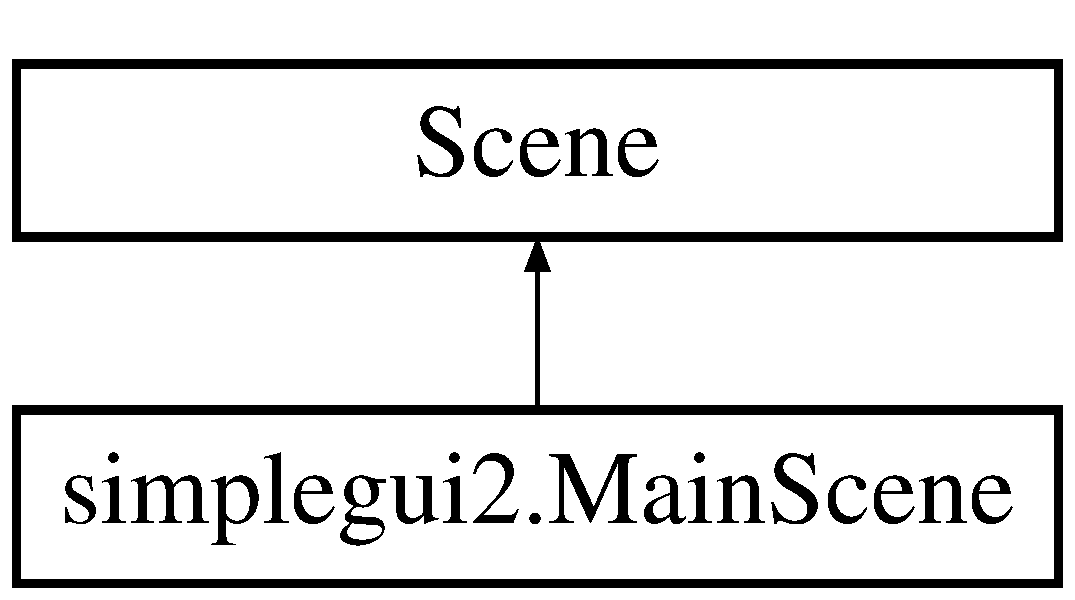
\includegraphics[height=2.000000cm]{classsimplegui2_1_1_main_scene}
\end{center}
\end{figure}
\subsection*{Public Member Functions}
\begin{DoxyCompactItemize}
\item 
\hypertarget{classsimplegui2_1_1_main_scene_a512bd8ab19046ed7a2fd655bc5bd025d}{def {\bfseries convert\-States}}\label{classsimplegui2_1_1_main_scene_a512bd8ab19046ed7a2fd655bc5bd025d}

\item 
\hypertarget{classsimplegui2_1_1_main_scene_ab8ba40320257851c4bb70a20c523269c}{def {\bfseries edit\-S\-Box}}\label{classsimplegui2_1_1_main_scene_ab8ba40320257851c4bb70a20c523269c}

\item 
\hypertarget{classsimplegui2_1_1_main_scene_a9e6debd72f75e89001ddab14eb52ed0f}{def {\bfseries run\-Round\-Keys}}\label{classsimplegui2_1_1_main_scene_a9e6debd72f75e89001ddab14eb52ed0f}

\item 
\hypertarget{classsimplegui2_1_1_main_scene_aa3fee479905df6d8522e89f31ffe8b5d}{def {\bfseries run\-Sub\-Bytes}}\label{classsimplegui2_1_1_main_scene_aa3fee479905df6d8522e89f31ffe8b5d}

\item 
\hypertarget{classsimplegui2_1_1_main_scene_a40656a24001ca03ac64df1228eb4581c}{def {\bfseries run\-Shift\-Rows}}\label{classsimplegui2_1_1_main_scene_a40656a24001ca03ac64df1228eb4581c}

\item 
\hypertarget{classsimplegui2_1_1_main_scene_ae49a81069e085a2dcf463b71119d5f2a}{def {\bfseries run\-Mix\-Columns}}\label{classsimplegui2_1_1_main_scene_ae49a81069e085a2dcf463b71119d5f2a}

\item 
\hypertarget{classsimplegui2_1_1_main_scene_a223abaad412e5f2c14808fd743344979}{def {\bfseries run\-Round}}\label{classsimplegui2_1_1_main_scene_a223abaad412e5f2c14808fd743344979}

\item 
\hypertarget{classsimplegui2_1_1_main_scene_a9250b1d513c66c5e7f1b7fe9c9452319}{def {\bfseries switch\-Key\-Plaintext\-Mode}}\label{classsimplegui2_1_1_main_scene_a9250b1d513c66c5e7f1b7fe9c9452319}

\item 
\hypertarget{classsimplegui2_1_1_main_scene_a62cb7fad67dbd5850ca9c922946458b2}{def {\bfseries show\-Entropy}}\label{classsimplegui2_1_1_main_scene_a62cb7fad67dbd5850ca9c922946458b2}

\item 
\hypertarget{classsimplegui2_1_1_main_scene_a337a884962532b842532071059891ce3}{def {\bfseries on\-Button\-Click}}\label{classsimplegui2_1_1_main_scene_a337a884962532b842532071059891ce3}

\item 
def \hyperlink{classsimplegui2_1_1_main_scene_ae741040ea754603bde928e92c73ce47a}{update\-View}
\item 
\hypertarget{classsimplegui2_1_1_main_scene_a533f53021aaf67dc23b066691036f946}{def {\bfseries histogram\-On\-View}}\label{classsimplegui2_1_1_main_scene_a533f53021aaf67dc23b066691036f946}

\item 
\hypertarget{classsimplegui2_1_1_main_scene_af277708f88c4aeff957509ce6872da43}{def {\bfseries punch\-Card\-On\-View}}\label{classsimplegui2_1_1_main_scene_af277708f88c4aeff957509ce6872da43}

\item 
\hypertarget{classsimplegui2_1_1_main_scene_ac8d7e0bb44f2128699c53e695465f828}{def {\bfseries bit\-Change\-On\-View}}\label{classsimplegui2_1_1_main_scene_ac8d7e0bb44f2128699c53e695465f828}

\item 
\hypertarget{classsimplegui2_1_1_main_scene_ae4e6b425653416ced6a5960aa8782bda}{def {\bfseries update\-Middle\-Column}}\label{classsimplegui2_1_1_main_scene_ae4e6b425653416ced6a5960aa8782bda}

\item 
def \hyperlink{classsimplegui2_1_1_main_scene_aaf3f84504c3d81259b958dda5310dc3c}{update\-Left\-Column}
\item 
def \hyperlink{classsimplegui2_1_1_main_scene_ac350e2bf2b7173ad136a0a95927b92f8}{update\-Right\-Column}
\item 
def \hyperlink{classsimplegui2_1_1_main_scene_ac8265bd3c200a716c923d0863a7483a2}{update\-Columns}
\item 
def \hyperlink{classsimplegui2_1_1_main_scene_a990a6cacd6e0477e034698d66b7b1142}{on\-Text\-Changed}
\item 
\hypertarget{classsimplegui2_1_1_main_scene_aa43b0159bd5355d2d3c826660f0c31e0}{def {\bfseries moo\-\_\-changed}}\label{classsimplegui2_1_1_main_scene_aa43b0159bd5355d2d3c826660f0c31e0}

\item 
\hypertarget{classsimplegui2_1_1_main_scene_ae2c46b1bb1991499dc647a97819cf5c2}{def {\bfseries round\-\_\-number\-\_\-changed}}\label{classsimplegui2_1_1_main_scene_ae2c46b1bb1991499dc647a97819cf5c2}

\item 
\hypertarget{classsimplegui2_1_1_main_scene_ab216549c93167d5a91f6107e9f30677f}{def {\bfseries expanded\-\_\-key\-\_\-size\-\_\-changed}}\label{classsimplegui2_1_1_main_scene_ab216549c93167d5a91f6107e9f30677f}

\item 
\hypertarget{classsimplegui2_1_1_main_scene_accf713c53fe35754a13987046389dce6}{def {\bfseries visualization\-\_\-changed}}\label{classsimplegui2_1_1_main_scene_accf713c53fe35754a13987046389dce6}

\item 
\hypertarget{classsimplegui2_1_1_main_scene_a5540717c415c66d3b3cdd66dfe142738}{def {\bfseries draw\-Top\-Bar}}\label{classsimplegui2_1_1_main_scene_a5540717c415c66d3b3cdd66dfe142738}

\item 
\hypertarget{classsimplegui2_1_1_main_scene_a62b6ab5f0d0449bd22d26afdc43c694f}{def {\bfseries draw\-Bottom\-Bar}}\label{classsimplegui2_1_1_main_scene_a62b6ab5f0d0449bd22d26afdc43c694f}

\item 
def \hyperlink{classsimplegui2_1_1_main_scene_abf459214036e594e6a157f2c1e50353d}{draw\-Lines\-For\-Grid}
\item 
\hypertarget{classsimplegui2_1_1_main_scene_aa036f33881a7f90541e17f812c7ce7fd}{def {\bfseries load\-\_\-image}}\label{classsimplegui2_1_1_main_scene_aa036f33881a7f90541e17f812c7ce7fd}

\item 
def \hyperlink{classsimplegui2_1_1_main_scene_a44aaf86b69d60fed3ed7971e6da2f0ff}{draw\-Left\-Column}
\item 
def \hyperlink{classsimplegui2_1_1_main_scene_ae41066730d48873984d89c0c42e6ea65}{draw\-Right\-Column}
\item 
def \hyperlink{classsimplegui2_1_1_main_scene_a643ddd077da213c2c52fbd5ad05beaef}{draw\-Center\-Column}
\item 
\hypertarget{classsimplegui2_1_1_main_scene_ad3a59ec0915e8eac0645de57e05ef742}{def {\bfseries history\-Forward}}\label{classsimplegui2_1_1_main_scene_ad3a59ec0915e8eac0645de57e05ef742}

\item 
\hypertarget{classsimplegui2_1_1_main_scene_a1bb7d4371a558fd8bdc077fe298e5545}{def {\bfseries history\-Backward}}\label{classsimplegui2_1_1_main_scene_a1bb7d4371a558fd8bdc077fe298e5545}

\item 
\hypertarget{classsimplegui2_1_1_main_scene_a6e393f1c44c5630cd9aceba0f70fe021}{def {\bfseries print\-History}}\label{classsimplegui2_1_1_main_scene_a6e393f1c44c5630cd9aceba0f70fe021}

\item 
\hypertarget{classsimplegui2_1_1_main_scene_ae98d95b9a339e4f6c031b4e3a6ec5d6c}{def {\bfseries add\-Point\-In\-History}}\label{classsimplegui2_1_1_main_scene_ae98d95b9a339e4f6c031b4e3a6ec5d6c}

\item 
\hypertarget{classsimplegui2_1_1_main_scene_a4f07584c7a7fd5afe2ff6c43d081c40d}{def {\bfseries clear\-History}}\label{classsimplegui2_1_1_main_scene_a4f07584c7a7fd5afe2ff6c43d081c40d}

\item 
\hypertarget{classsimplegui2_1_1_main_scene_a12a186ce2e8a1d201fd904dd17a887ba}{def {\bfseries \-\_\-\-\_\-init\-\_\-\-\_\-}}\label{classsimplegui2_1_1_main_scene_a12a186ce2e8a1d201fd904dd17a887ba}

\item 
\hypertarget{classsimplegui2_1_1_main_scene_af0d09e7b92c32cd567cc47464b0ba9d5}{def {\bfseries layout}}\label{classsimplegui2_1_1_main_scene_af0d09e7b92c32cd567cc47464b0ba9d5}

\item 
\hypertarget{classsimplegui2_1_1_main_scene_a0e488df64a1ad3eeb8b9a91f5749823e}{def {\bfseries update}}\label{classsimplegui2_1_1_main_scene_a0e488df64a1ad3eeb8b9a91f5749823e}

\item 
\hypertarget{classsimplegui2_1_1_main_scene_a080a9fa6536a29a124eebd15ef99190e}{def {\bfseries get\-R\-G\-B}}\label{classsimplegui2_1_1_main_scene_a080a9fa6536a29a124eebd15ef99190e}

\end{DoxyCompactItemize}
\subsection*{Public Attributes}
\begin{DoxyCompactItemize}
\item 
\hypertarget{classsimplegui2_1_1_main_scene_a3c02eda8911b4354745c7fe32f8c90e0}{{\bfseries ptk\-Mode}}\label{classsimplegui2_1_1_main_scene_a3c02eda8911b4354745c7fe32f8c90e0}

\item 
\hypertarget{classsimplegui2_1_1_main_scene_a3c4434194d04a83467d3a685c6751b7f}{{\bfseries lb\-Entry}}\label{classsimplegui2_1_1_main_scene_a3c4434194d04a83467d3a685c6751b7f}

\item 
\hypertarget{classsimplegui2_1_1_main_scene_a8965a4ec239efb79884e84669125d565}{{\bfseries lt\-Entry}}\label{classsimplegui2_1_1_main_scene_a8965a4ec239efb79884e84669125d565}

\item 
\hypertarget{classsimplegui2_1_1_main_scene_a12bc85a82caa5aff90b7f191a796a59d}{{\bfseries lm\-Entry}}\label{classsimplegui2_1_1_main_scene_a12bc85a82caa5aff90b7f191a796a59d}

\item 
\hypertarget{classsimplegui2_1_1_main_scene_a1d85aff9a2fa7b49490724165d0d3c07}{{\bfseries original\-Entropy}}\label{classsimplegui2_1_1_main_scene_a1d85aff9a2fa7b49490724165d0d3c07}

\item 
\hypertarget{classsimplegui2_1_1_main_scene_acf31e6c853ef7d3445adb8b91fa588ba}{{\bfseries states\-Entropy}}\label{classsimplegui2_1_1_main_scene_acf31e6c853ef7d3445adb8b91fa588ba}

\item 
\hypertarget{classsimplegui2_1_1_main_scene_a9c18ff79726e76cbed54037dd836a200}{{\bfseries crypts\-Entropy}}\label{classsimplegui2_1_1_main_scene_a9c18ff79726e76cbed54037dd836a200}

\item 
\hypertarget{classsimplegui2_1_1_main_scene_a3d01c259a330f498181c48959f5c86a1}{{\bfseries cleartext}}\label{classsimplegui2_1_1_main_scene_a3d01c259a330f498181c48959f5c86a1}

\item 
\hypertarget{classsimplegui2_1_1_main_scene_a4be17c3750458392c0058517db71a3b9}{{\bfseries ciph}}\label{classsimplegui2_1_1_main_scene_a4be17c3750458392c0058517db71a3b9}

\item 
\hypertarget{classsimplegui2_1_1_main_scene_acc8ffbe63e9f7177a4629fef8b88beed}{{\bfseries visualization}}\label{classsimplegui2_1_1_main_scene_acc8ffbe63e9f7177a4629fef8b88beed}

\item 
\hypertarget{classsimplegui2_1_1_main_scene_a992480f7d94639b79aa82a19a541ad11}{{\bfseries operation\-Mode}}\label{classsimplegui2_1_1_main_scene_a992480f7d94639b79aa82a19a541ad11}

\item 
\hypertarget{classsimplegui2_1_1_main_scene_a9cbb42c0edac9d1b328fb25476195951}{{\bfseries key\-Size}}\label{classsimplegui2_1_1_main_scene_a9cbb42c0edac9d1b328fb25476195951}

\item 
\hypertarget{classsimplegui2_1_1_main_scene_a55fe5a0ecc375e5ac28ccf249cf39387}{{\bfseries plaintextone\-\_\-imageview}}\label{classsimplegui2_1_1_main_scene_a55fe5a0ecc375e5ac28ccf249cf39387}

\item 
\hypertarget{classsimplegui2_1_1_main_scene_ac1edcf6a8f80f1fdbef0685ac664745d}{{\bfseries plaintexttwo\-\_\-imageview}}\label{classsimplegui2_1_1_main_scene_ac1edcf6a8f80f1fdbef0685ac664745d}

\item 
\hypertarget{classsimplegui2_1_1_main_scene_abd39b51e4c51cd13353c7ecbc28ed6ed}{{\bfseries lefttop\-\_\-textfield}}\label{classsimplegui2_1_1_main_scene_abd39b51e4c51cd13353c7ecbc28ed6ed}

\item 
\hypertarget{classsimplegui2_1_1_main_scene_a9e1e997632819c75594d064d525e804a}{{\bfseries leftbottom\-\_\-textfield}}\label{classsimplegui2_1_1_main_scene_a9e1e997632819c75594d064d525e804a}

\item 
\hypertarget{classsimplegui2_1_1_main_scene_a19ac77092a1ed6870bdf35bff235a783}{{\bfseries leftmiddle\-\_\-textfield}}\label{classsimplegui2_1_1_main_scene_a19ac77092a1ed6870bdf35bff235a783}

\item 
\hypertarget{classsimplegui2_1_1_main_scene_aa67815fee66b1671b13861c93fe0967e}{{\bfseries cipherone\-\_\-imageview}}\label{classsimplegui2_1_1_main_scene_aa67815fee66b1671b13861c93fe0967e}

\item 
\hypertarget{classsimplegui2_1_1_main_scene_a6463a7d9e584ac5206931ef59109f5f6}{{\bfseries ciphertwo\-\_\-imageview}}\label{classsimplegui2_1_1_main_scene_a6463a7d9e584ac5206931ef59109f5f6}

\item 
\hypertarget{classsimplegui2_1_1_main_scene_aa51999dbff085e261905ab761c69c6ac}{{\bfseries currentone\-\_\-imageview}}\label{classsimplegui2_1_1_main_scene_aa51999dbff085e261905ab761c69c6ac}

\item 
\hypertarget{classsimplegui2_1_1_main_scene_ad35c846ffbe75caa0ac30a25c5357a49}{{\bfseries currenttwo\-\_\-imageview}}\label{classsimplegui2_1_1_main_scene_ad35c846ffbe75caa0ac30a25c5357a49}

\item 
\hypertarget{classsimplegui2_1_1_main_scene_acd6101f267e7aef628af7bcd7e07ccae}{{\bfseries future}}\label{classsimplegui2_1_1_main_scene_acd6101f267e7aef628af7bcd7e07ccae}

\item 
\hypertarget{classsimplegui2_1_1_main_scene_ae11929d10ae440f5cb4aecfefc02fea6}{{\bfseries history}}\label{classsimplegui2_1_1_main_scene_ae11929d10ae440f5cb4aecfefc02fea6}

\item 
\hypertarget{classsimplegui2_1_1_main_scene_af7ce77f8a8ed2f81d1df9d12ed7d2e13}{{\bfseries moo}}\label{classsimplegui2_1_1_main_scene_af7ce77f8a8ed2f81d1df9d12ed7d2e13}

\item 
\hypertarget{classsimplegui2_1_1_main_scene_a5c194f4e8eb948fbdca30d1ef4b3e37b}{{\bfseries cypherkey}}\label{classsimplegui2_1_1_main_scene_a5c194f4e8eb948fbdca30d1ef4b3e37b}

\item 
\hypertarget{classsimplegui2_1_1_main_scene_a2874ca965ec158410b9aafedc92cce34}{{\bfseries iv}}\label{classsimplegui2_1_1_main_scene_a2874ca965ec158410b9aafedc92cce34}

\item 
\hypertarget{classsimplegui2_1_1_main_scene_ab985f4fcd69ce112ad0379b3db0fb5c3}{{\bfseries label\-\_\-height}}\label{classsimplegui2_1_1_main_scene_ab985f4fcd69ce112ad0379b3db0fb5c3}

\item 
\hypertarget{classsimplegui2_1_1_main_scene_aeafa1283e41e1a238c8ac17b5060573e}{{\bfseries button\-Bar\-Bottom}}\label{classsimplegui2_1_1_main_scene_aeafa1283e41e1a238c8ac17b5060573e}

\item 
\hypertarget{classsimplegui2_1_1_main_scene_a15e46be8ef02bfae376eb1810f1aaefe}{{\bfseries column\-Width}}\label{classsimplegui2_1_1_main_scene_a15e46be8ef02bfae376eb1810f1aaefe}

\item 
\hypertarget{classsimplegui2_1_1_main_scene_a385fdec756c9d6ff3fcb8648f61b3962}{{\bfseries middle\-Bar\-Y}}\label{classsimplegui2_1_1_main_scene_a385fdec756c9d6ff3fcb8648f61b3962}

\item 
\hypertarget{classsimplegui2_1_1_main_scene_ad80abde9a66a9c43201f278a1663f290}{{\bfseries empty}}\label{classsimplegui2_1_1_main_scene_ad80abde9a66a9c43201f278a1663f290}

\end{DoxyCompactItemize}
\subsection*{Static Public Attributes}
\begin{DoxyCompactItemize}
\item 
\hypertarget{classsimplegui2_1_1_main_scene_a461593d8f0e6510859042c3b06ee5d68}{tuple {\bfseries aes} = \hyperlink{classslowaes_1_1_a_e_s}{slowaes.\-A\-E\-S}()}\label{classsimplegui2_1_1_main_scene_a461593d8f0e6510859042c3b06ee5d68}

\item 
\hypertarget{classsimplegui2_1_1_main_scene_ac295cbd5f6e3e052232f6490ed2a68cf}{tuple {\bfseries aesmoo} = \hyperlink{classslowaes_1_1_a_e_s_mode_of_operation}{slowaes.\-A\-E\-S\-Mode\-Of\-Operation}()}\label{classsimplegui2_1_1_main_scene_ac295cbd5f6e3e052232f6490ed2a68cf}

\end{DoxyCompactItemize}


\subsection{Member Function Documentation}
\hypertarget{classsimplegui2_1_1_main_scene_a643ddd077da213c2c52fbd5ad05beaef}{\index{simplegui2\-::\-Main\-Scene@{simplegui2\-::\-Main\-Scene}!draw\-Center\-Column@{draw\-Center\-Column}}
\index{draw\-Center\-Column@{draw\-Center\-Column}!simplegui2::MainScene@{simplegui2\-::\-Main\-Scene}}
\subsubsection[{draw\-Center\-Column}]{\setlength{\rightskip}{0pt plus 5cm}def simplegui2.\-Main\-Scene.\-draw\-Center\-Column (
\begin{DoxyParamCaption}
\item[{}]{self}
\end{DoxyParamCaption}
)}}\label{classsimplegui2_1_1_main_scene_a643ddd077da213c2c52fbd5ad05beaef}
\begin{DoxyVerb}    This draws the center column.
    This will be the current cipher keys and a slider at the bottom
    for history.
\end{DoxyVerb}
 \hypertarget{classsimplegui2_1_1_main_scene_a44aaf86b69d60fed3ed7971e6da2f0ff}{\index{simplegui2\-::\-Main\-Scene@{simplegui2\-::\-Main\-Scene}!draw\-Left\-Column@{draw\-Left\-Column}}
\index{draw\-Left\-Column@{draw\-Left\-Column}!simplegui2::MainScene@{simplegui2\-::\-Main\-Scene}}
\subsubsection[{draw\-Left\-Column}]{\setlength{\rightskip}{0pt plus 5cm}def simplegui2.\-Main\-Scene.\-draw\-Left\-Column (
\begin{DoxyParamCaption}
\item[{}]{self}
\end{DoxyParamCaption}
)}}\label{classsimplegui2_1_1_main_scene_a44aaf86b69d60fed3ed7971e6da2f0ff}
\begin{DoxyVerb}    This draws the left column.
    This column consists of two surfaces showing the initial string,
    along input text boxes for the strings.
\end{DoxyVerb}
 \hypertarget{classsimplegui2_1_1_main_scene_abf459214036e594e6a157f2c1e50353d}{\index{simplegui2\-::\-Main\-Scene@{simplegui2\-::\-Main\-Scene}!draw\-Lines\-For\-Grid@{draw\-Lines\-For\-Grid}}
\index{draw\-Lines\-For\-Grid@{draw\-Lines\-For\-Grid}!simplegui2::MainScene@{simplegui2\-::\-Main\-Scene}}
\subsubsection[{draw\-Lines\-For\-Grid}]{\setlength{\rightskip}{0pt plus 5cm}def simplegui2.\-Main\-Scene.\-draw\-Lines\-For\-Grid (
\begin{DoxyParamCaption}
\item[{}]{self}
\end{DoxyParamCaption}
)}}\label{classsimplegui2_1_1_main_scene_abf459214036e594e6a157f2c1e50353d}
\begin{DoxyVerb}    This draws the grid lines.
    This includes the two lines going top to bottom for each column.
    This also includes the bar below the buttons at the top and the
    middle horizontal line separating the two plain texts, cipher texts
    and current progress.
\end{DoxyVerb}
 \hypertarget{classsimplegui2_1_1_main_scene_ae41066730d48873984d89c0c42e6ea65}{\index{simplegui2\-::\-Main\-Scene@{simplegui2\-::\-Main\-Scene}!draw\-Right\-Column@{draw\-Right\-Column}}
\index{draw\-Right\-Column@{draw\-Right\-Column}!simplegui2::MainScene@{simplegui2\-::\-Main\-Scene}}
\subsubsection[{draw\-Right\-Column}]{\setlength{\rightskip}{0pt plus 5cm}def simplegui2.\-Main\-Scene.\-draw\-Right\-Column (
\begin{DoxyParamCaption}
\item[{}]{self}
\end{DoxyParamCaption}
)}}\label{classsimplegui2_1_1_main_scene_ae41066730d48873984d89c0c42e6ea65}
\begin{DoxyVerb}    This draws the right column.
    This will be the normal result of the plain texts if ran normally
    through AES.
\end{DoxyVerb}
 \hypertarget{classsimplegui2_1_1_main_scene_a990a6cacd6e0477e034698d66b7b1142}{\index{simplegui2\-::\-Main\-Scene@{simplegui2\-::\-Main\-Scene}!on\-Text\-Changed@{on\-Text\-Changed}}
\index{on\-Text\-Changed@{on\-Text\-Changed}!simplegui2::MainScene@{simplegui2\-::\-Main\-Scene}}
\subsubsection[{on\-Text\-Changed}]{\setlength{\rightskip}{0pt plus 5cm}def simplegui2.\-Main\-Scene.\-on\-Text\-Changed (
\begin{DoxyParamCaption}
\item[{}]{self, }
\item[{}]{tf, }
\item[{}]{text}
\end{DoxyParamCaption}
)}}\label{classsimplegui2_1_1_main_scene_a990a6cacd6e0477e034698d66b7b1142}
\begin{DoxyVerb}tf is the TextField object.
    Text is the text the TextField was changed to.
\end{DoxyVerb}
 \hypertarget{classsimplegui2_1_1_main_scene_ac8265bd3c200a716c923d0863a7483a2}{\index{simplegui2\-::\-Main\-Scene@{simplegui2\-::\-Main\-Scene}!update\-Columns@{update\-Columns}}
\index{update\-Columns@{update\-Columns}!simplegui2::MainScene@{simplegui2\-::\-Main\-Scene}}
\subsubsection[{update\-Columns}]{\setlength{\rightskip}{0pt plus 5cm}def simplegui2.\-Main\-Scene.\-update\-Columns (
\begin{DoxyParamCaption}
\item[{}]{self}
\end{DoxyParamCaption}
)}}\label{classsimplegui2_1_1_main_scene_ac8265bd3c200a716c923d0863a7483a2}
\begin{DoxyVerb}This updates all the columns.  Redraws the left, right, and center. \end{DoxyVerb}
 \hypertarget{classsimplegui2_1_1_main_scene_aaf3f84504c3d81259b958dda5310dc3c}{\index{simplegui2\-::\-Main\-Scene@{simplegui2\-::\-Main\-Scene}!update\-Left\-Column@{update\-Left\-Column}}
\index{update\-Left\-Column@{update\-Left\-Column}!simplegui2::MainScene@{simplegui2\-::\-Main\-Scene}}
\subsubsection[{update\-Left\-Column}]{\setlength{\rightskip}{0pt plus 5cm}def simplegui2.\-Main\-Scene.\-update\-Left\-Column (
\begin{DoxyParamCaption}
\item[{}]{self}
\end{DoxyParamCaption}
)}}\label{classsimplegui2_1_1_main_scene_aaf3f84504c3d81259b958dda5310dc3c}
\begin{DoxyVerb}This should update the left column \end{DoxyVerb}
 \hypertarget{classsimplegui2_1_1_main_scene_ac350e2bf2b7173ad136a0a95927b92f8}{\index{simplegui2\-::\-Main\-Scene@{simplegui2\-::\-Main\-Scene}!update\-Right\-Column@{update\-Right\-Column}}
\index{update\-Right\-Column@{update\-Right\-Column}!simplegui2::MainScene@{simplegui2\-::\-Main\-Scene}}
\subsubsection[{update\-Right\-Column}]{\setlength{\rightskip}{0pt plus 5cm}def simplegui2.\-Main\-Scene.\-update\-Right\-Column (
\begin{DoxyParamCaption}
\item[{}]{self}
\end{DoxyParamCaption}
)}}\label{classsimplegui2_1_1_main_scene_ac350e2bf2b7173ad136a0a95927b92f8}
\begin{DoxyVerb}This should update the right column \end{DoxyVerb}
 \hypertarget{classsimplegui2_1_1_main_scene_ae741040ea754603bde928e92c73ce47a}{\index{simplegui2\-::\-Main\-Scene@{simplegui2\-::\-Main\-Scene}!update\-View@{update\-View}}
\index{update\-View@{update\-View}!simplegui2::MainScene@{simplegui2\-::\-Main\-Scene}}
\subsubsection[{update\-View}]{\setlength{\rightskip}{0pt plus 5cm}def simplegui2.\-Main\-Scene.\-update\-View (
\begin{DoxyParamCaption}
\item[{}]{self, }
\item[{}]{text, }
\item[{}]{view, }
\item[{}]{size}
\end{DoxyParamCaption}
)}}\label{classsimplegui2_1_1_main_scene_ae741040ea754603bde928e92c73ce47a}
\begin{DoxyVerb}    This method accepts a string, cipher/plain text (text), and updates the view (view) given.
    The size is a tuple (#,#) that is the resulting size.
\end{DoxyVerb}
 

The documentation for this class was generated from the following file\-:\begin{DoxyCompactItemize}
\item 
simplegui2.\-py\end{DoxyCompactItemize}

\hypertarget{classsetup_1_1pygame2exe}{\section{setup.\-pygame2exe Class Reference}
\label{classsetup_1_1pygame2exe}\index{setup.\-pygame2exe@{setup.\-pygame2exe}}
}
Inheritance diagram for setup.\-pygame2exe\-:\begin{figure}[H]
\begin{center}
\leavevmode
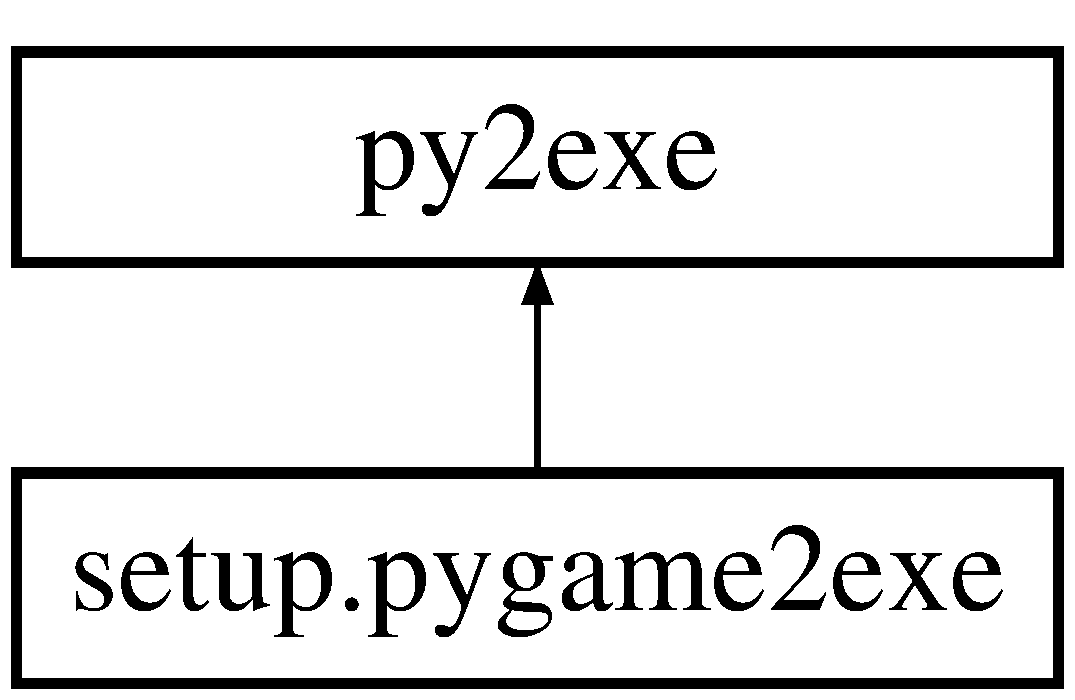
\includegraphics[height=2.000000cm]{classsetup_1_1pygame2exe}
\end{center}
\end{figure}


The documentation for this class was generated from the following file\-:\begin{DoxyCompactItemize}
\item 
setup.\-py\end{DoxyCompactItemize}

%--- End generated contents ---

% Index
\newpage
\phantomsection
\addcontentsline{toc}{part}{Index}
\printindex

\end{document}
